\documentclass[10pt]{article}
\usepackage[a4paper,margin=25mm]{geometry}
\usepackage{amsmath,amssymb,amsthm,booktabs,array}
\usepackage[T1]{fontenc}
\usepackage{mathptmx}
\usepackage{courier}
\usepackage{microtype}
\usepackage{graphicx}
\usepackage[font=small,labelfont=bf]{caption}
\captionsetup[table]{position=top,skip=9pt}
\captionsetup[figure]{skip=8pt}
\setlength{\textfloatsep}{20pt plus 4pt minus 2pt}
\setlength{\intextsep}{18pt plus 4pt minus 2pt}
\setlength{\floatsep}{16pt plus 4pt minus 2pt}
\renewcommand{\arraystretch}{1.12}
\usepackage[numbers,square,sort&compress]{natbib}
\usepackage[colorlinks=true,allcolors=blue]{hyperref}
\newcommand{\dd}{\,\mathrm{d}}
\newcommand{\R}{\mathbb{R}}
\newtheorem{proposition}{Proposition}
\title{\fontsize{16}{20}\selectfont\bfseries
Geometry-consistent conservative transfer of potential-flow states
to an embedded-boundary volume-of-fluid solver}
\ifdefined\BlindReview
\author{Anonymous manuscript}
\else
\author{Saveliy Baturin\\\small Independent Researcher, Moscow, Russia\\
\small\href{mailto:saveliy.xo@gmail.com}{saveliy.xo@gmail.com}\\
\small ORCID: \href{https://orcid.org/0009-0005-4410-9520}{0009-0005-4410-9520}}
\fi
\date{}
\begin{document}
\maketitle

\begin{abstract}
Transferring a potential-flow state to a volume-of-fluid (VOF) solver
requires accurate liquid-cell velocities on the geometry used by the
receiver. We reconstruct liquid-cell moments by integrating a harmonic
streamfunction over the polygonal cell boundary. For thin strips beneath a
flat free surface, a boundary-normal extension uses one trace for the
physical edge and its neighbouring Cartesian edge. Their common trace
error cancels within the extension; a smooth blend connects it to the
interior reconstruction. We give an error bound for the combined operator
and test it against analytic cell means. In 21
initial-field cases, global velocity error is 2.71--32.07 times smaller
than for a bilinear control using the same streamfunction. In subsequent
smooth-wave calculations, the method also reduces the difference from
same-grid numerical trajectories started with exact cell means. Against an
independent linear two-fluid wave, it reduces endpoint physical
surface-profile error by 2.81--5.49\% on two grids when receiver velocity
assignment is held fixed.
\end{abstract}
\noindent\textbf{Keywords:} conservative transfer; boundary integral method;
streamfunction; cut cells; embedded boundaries; volume of fluid.

\section{Introduction}
Potential-flow boundary-integral-equation (BIE) methods represent strongly deformed free
surfaces efficiently while the liquid remains irrotational and its boundary
does not intersect itself. A two-phase field solver can subsequently represent
flows outside that model class. Potential-to-field coupling is established:
\citet{lachaume} combined boundary-element (BEM) and VOF methods for waves on slopes,
and \citet{colicchio} developed BEM--level-set domain
decomposition for strongly deformed and fragmented interfaces. More recent
hybrid wave calculations include experimental comparisons and investigations
of turbulence closures~\citep{zhang}. We focus on transferring a
potential-flow state to a field solver.

Compatibility between velocity data and transport discretizations is a
separate numerical problem~\citep{sun}. Conservative remapping using geometric
integration is well established~\citep{ullrich}, and streamfunction-based
divergence-free interpolation has been developed for cut-cell fluid grids
\citep{chang,curlflow}. Curl-Flow reconstructs a potential from staggered-grid
velocities to obtain pointwise incompressible interpolation and enforce solid
boundary conditions. Our input is instead a potential-flow boundary state,
and the output of interest is the liquid-volume mean in each receiving cell.
Taylor reconstruction combined with geometric moments also
supports high-order embedded-boundary discretisations, including an unsteady
Stokes method~\citep{overton}. Here the physical trace and the adjacent
Cartesian edge must be represented consistently in thin liquid strips.
Table~\ref{tab:related-methods} compares the inputs, outputs, and target
properties of these related constructions.
\begin{table}[tbp]\centering\small
\caption{Related numerical constructions and the transfer problem considered here.
The rows compare their inputs and objectives; they are not a ranking of accuracy.}
\label{tab:related-methods}
\begin{tabular}{@{}>{\raggedright\arraybackslash}p{0.17\linewidth}
                  >{\raggedright\arraybackslash}p{0.23\linewidth}
                  >{\raggedright\arraybackslash}p{0.25\linewidth}
                  >{\raggedright\arraybackslash}p{0.25\linewidth}@{}}
\toprule
Construction & Input and output & Main property & Relation to the present problem\\
\midrule
Conservative remapping~\citep{ullrich}
& Discretised scalar fields on a source mesh to fields on a target mesh.
& Global integral and constant fields; monotonicity for suitable maps.
& Mesh-to-mesh transfer of scalar fields, rather than liquid velocity means from boundary data.\\[5pt]
Curl-Flow~\citep{curlflow}
& Discretely divergence-free staggered velocities to a continuous velocity interpolant.
& Pointwise incompressibility and solid-wall non-penetration.
& Reconstructs a vector potential from grid velocities; the target is pointwise interpolation.\\[5pt]
High-order embedded-boundary Stokes method~\citep{overton}
& Cell data and boundary conditions to a finite-volume time evolution.
& High-order spatial operators with an approximate incompressibility projection.
& Uses geometric moments and Taylor reconstruction to discretise a flow solver.\\[5pt]
Present construction
& Potential-flow boundary data to liquid-cell velocity means on receiver polygons.
& Shared-edge liquid-moment balance; cancellation of common trace error in flat strips.
& Matches the physical and adjacent Cartesian edge averages before division by strip thickness.\\
\bottomrule
\end{tabular}
\end{table}

We combine a BIE-derived liquid reconstruction with phase-volume moments
on the geometry used by the receiver. This requires care with three
distinctions: Cartesian face averages differ from liquid-cell means;
Cartesian divergence cancellation does not guarantee zero embedded-volume
flux divergence after loading; and independently clipped polygons may differ
from the receiver's solid geometry.
The liquid-phase mean also differs from a density-weighted mixture
velocity in a cell containing both phases; the independent two-fluid
benchmark tests this receiver assignment separately.

Consistency of mass and momentum transport is especially important at large
density contrasts. Earlier volume-tracking work~\citep{rudman} and subsequent
staggered-grid VOF schemes~\citep{arrufat} address this issue in the advection
operator. Conservative VOF transport itself also depends on how the velocity
field and directional stretching are represented~\citep{weymouth}. Here we
study the preceding initialisation step: a liquid moment and a mixture
moment represent different quantities even when both are conservative.
The density-weighted assignment used below is a standard projection; the
factorial experiment measures its contribution separately from that of
the new boundary extension.

The general construction integrates liquid moments on receiver-matched
polygons. Its internal edge contributions cancel by a standard discrete
Green identity; this provides conservation on the represented geometry.
The central accuracy improvement is narrower: for thin strips below a flat
free surface, a boundary-normal extension uses the same trace on the
physical and neighbouring Cartesian edges. This cancels the shared trace
error before division by strip thickness. We test that mechanism against
analytic cell means, propagated transfer error, and an independent physical
wave. Additional tests of the general polygonal operator on an overturning
state appear in Appendix~\ref{app:general-tests}.
The numerical scope is periodic, two-dimensional, square Cartesian grids,
an impermeable single-valued bed, and a resolved non-self-intersecting free
surface.

\section{Transfer problem}
Let $\Omega_\ell$ be the liquid region in a periodic strip of length $L$.
Its upper boundary $\Gamma_f$ may overturn and its bed $\Gamma_b$ is
single-valued. The source supplies potential and normal-derivative traces
for the harmonic problem
\begin{equation}
 \Delta\phi=0\quad\hbox{in }\Omega_\ell,\qquad
 \partial_n\phi=0\quad\hbox{on }\Gamma_b,\qquad
 \boldsymbol u=\nabla\phi.
\end{equation}
The tested source has zero background current. We check boundary-flux
compatibility before reconstructing the streamfunction and reject
incompatible source states.

For a square Cartesian cell $K$ of area $h^2$, define
\begin{equation}
 c_{s,K}=\frac{|K\cap\Omega_f|}{h^2},\qquad
 q_K=\frac{|K\cap\Omega_\ell|}{h^2},\qquad
 f_K=\frac{q_K}{c_{s,K}}\quad(c_{s,K}>0),
 \label{eq:fractions}
\end{equation}
where $\Omega_f$ is the non-solid domain. Thus $0\le q_K\le c_{s,K}\le1$.
The liquid mean velocity and its moment are
\begin{equation}
 \overline{\boldsymbol u}_{\ell,K}
   =\frac{1}{q_Kh^2}\int_{K\cap\Omega_\ell}\boldsymbol u\dd A,
 \qquad \boldsymbol m_K=q_Kh^2\overline{\boldsymbol u}_{\ell,K}.
 \label{eq:means}
\end{equation}
The density-normalised liquid momentum is $\boldsymbol M_h=\sum_K\boldsymbol m_K$.
Every liquid-containing cell enters this sum, including small cut cells.
The quantity $\overline{\boldsymbol u}_{\ell,K}$ is distinct from both a
whole-cell mean and a MAC face average. Initial momentum is a transfer target;
it is not assumed constant during subsequent evolution under gravity and
boundary forces.

\section{Liquid streamfunction reconstruction}
Cartesian elliptic solvers with irregular Dirichlet boundaries are well
established; \citet{gibou}, for example, give a symmetric second-order
discretisation. We use the cut-distance scheme specified below.
We use the convention
\begin{equation}
 u=\partial_z\psi,\qquad w=-\partial_x\psi,\qquad \Delta\psi=0.
 \label{eq:psi}
\end{equation}
On a boundary parameterised by $\boldsymbol X(\alpha)$, the source normal
velocity fixes the tangential derivative of $\psi$, with its sign determined
by the boundary orientation. In counterclockwise liquid-boundary orientation,
with arc length $s$ and the outward normal, the convention in~\eqref{eq:psi}
gives $\partial_s\psi=\partial_n\phi$. The implementation uses periodic spectral
integration on the upper boundary and a constant bed trace. The relative
constant between the two boundary traces is fixed from the horizontal
momentum identity of the source. Compatibility of the vertical momentum
identities is checked independently. No velocity rescaling is applied afterward.

In particular, if both periodic boundary curves are traversed once with
net horizontal displacement $+L$ and the bed trace is zero, then
$M_x=\int_{\Gamma_f}\psi\dd x$. Adding a constant $C$ to the free-surface
trace changes this moment by $CL$, even for an overturning surface.
The relative trace constant is therefore fixed by the source horizontal
transport, whereas a common additive gauge on all boundaries leaves the
velocity and closed-cell moments unchanged.

The harmonic Dirichlet problem is solved only at liquid grid vertices. If the
distances to the left and right neighbouring values or boundary crossings are
$a_-$ and $a_+$, the horizontal second derivative is approximated by
\begin{equation}
 \frac{2}{a_-+a_+}
 \left(\frac{\psi_+-\psi_0}{a_+}
       -\frac{\psi_0-\psi_-}{a_-}\right).
 \label{eq:sw}
\end{equation}
The vertical expression is analogous. At a cut link, the prescribed
physical trace replaces the exterior unknown. This cut-distance matrix is
generally nonsymmetric; the implementation uses BiCGStab on CPU or restarted
GMRES on GPU and checks the true residual after solving.

Exterior vertices required by liquid-containing cells receive a short normal
Taylor continuation from the physical trace. The tested variant includes
the quadratic term, with the normal second derivative obtained from
harmonicity and boundary derivatives. A separate gas continuation then fills
the remaining region while holding all liquid-support vertices fixed. The
liquid solve and its moments are therefore unchanged by that gas completion.
This isolation is an initialisation property; it does not remove the physical
influence of gas during two-phase evolution.

\section{Shared-edge liquid moments}
\subsection{Green identity and edge quadrature}
Write $P_K=K\cap\Omega_{\ell,h}$ for the polygonal liquid portion of a cell.
Orient each exterior ring counterclockwise and each hole clockwise. Applying
Green's identity to~\eqref{eq:psi} gives
\begin{equation}
 \boldsymbol m_K=-\oint_{\partial P_K}\psi\,(\dd x,\dd z).
 \label{eq:green}
\end{equation}
For a directed straight edge from $A$ to $B$, let
$\boldsymbol\Delta=B-A$, $\psi_A,\psi_B$ be its endpoint values, and
$\boldsymbol g_A,\boldsymbol g_B$ their reconstructed gradients. The average
of the cubic Hermite interpolant along the edge is
\begin{equation}
 I_{AB}=\frac{\psi_A+\psi_B}{2}
       +\frac{(\boldsymbol g_A-\boldsymbol g_B)\cdot\boldsymbol\Delta}{12}.
 \label{eq:hermite}
\end{equation}
Its contribution to~\eqref{eq:green} is $-I_{AB}\boldsymbol\Delta$.
In the baseline operator, the physical-boundary trace is piecewise linear, so
the correction in~\eqref{eq:hermite} is omitted. This keeps the physical
trace integral identical to the one used to define the polygonal target.
Cartesian edges use the Hermite rule in both full and cut cells.
We call this \emph{Linear} (L). \emph{Hermite} (H) changes only the physical
trace to cubic Hermite integration. \emph{Matched} (M) also couples that
trace to the neighbouring Cartesian edge in a flat surface strip through
\eqref{eq:matched-jet} and the blend below. \emph{Bilinear} (B) takes the
curl of a piecewise-bilinear interpolant of the same solved streamfunction
and evaluates its liquid-polygon mean at the polygon centroid (the exact
mean of that affine velocity field). It does not use the liquid edge
integral. These names refer to transfer
variants, not to the later receiver velocity assignment.

At Cartesian vertices the gradients are centred differences of the completed
streamfunction, with second-order one-sided differences at artificial
vertical endpoints. At a physical-boundary intersection in the baseline operator, the trace value
and its two gradient components are linearly interpolated from the enclosing
source-boundary segment. Thus the edge rule uses source derivatives at
boundary intersections and grid derivatives at interior corners. The same
endpoint data are reused by adjacent cells.

\begin{proposition}[Discrete liquid-moment closure]
Suppose the liquid polygons form a conforming partition, every shared edge
uses the same scalar integral with opposite orientation in its adjacent
cells, and the periodic seam values match. Then the sum of the cell moments
computed from~\eqref{eq:green} equals the integral over the exterior physical
boundary of the polygonal liquid domain.
\end{proposition}
\begin{proof}
Sum the oriented edge contributions over all polygons. Every internal edge
appears twice with the same scalar integral and opposite directed edge
vector, so the two contributions cancel. Periodic seam contributions cancel
by the same argument. The remaining terms are precisely those on the
physical boundary. In floating-point arithmetic the statement holds up to
geometry and summation errors.
\end{proof}

This identity concerns the polygonal reconstruction. Agreement with the
continuous BIE momentum also depends on the boundary representation and
source accuracy. The same edge rule must be used in full and cut cells for
shared contributions to cancel.

\subsection{Gauge subtraction and small-cell limitations}
For any constant $c_K$, replacing $\psi$ by $\psi-c_K$ in a closed-cell
boundary integral leaves the moment unchanged because
$\oint_{\partial P_K}(\dd x,\dd z)=0$. The implementation uses a local
constant to reduce cancellation when a small polygon is evaluated against a
large streamfunction gauge.

Division by $q_Kh^2$ in~\eqref{eq:means} is nevertheless a distinct source of
sensitivity. For a fixed geometry, an absolute moment error $\delta\boldsymbol
m_K$ induces a mean-velocity error
$\delta\overline{\boldsymbol u}_{\ell,K}=\delta\boldsymbol m_K/(q_Kh^2)$.
Global closure therefore gives no uniform small-cell accuracy estimate.
We report both phase-volume-weighted errors and errors by liquid fraction.

A direct perturbation bound makes this sensitivity explicit. Let
$\delta I_e$ be the error in the scalar edge average used in
\eqref{eq:green}, on the same polygon as the reference, and let $\ell_e$
be its edge length. The triangle inequality yields
\begin{equation}
 \|\delta\overline{\boldsymbol u}_{\ell,K}\|_2
 \le \frac{\sum_{e\subset\partial P_K}\ell_e|\delta I_e|}{q_Kh^2}
 \le \frac{|\partial P_K|}{q_Kh^2}\max_e|\delta I_e|.
 \label{eq:sliver-bound}
\end{equation}
For fixed geometry, this bound shows how edge-average errors grow when
divided by a small liquid area. It does not bound the subsequent flow error.

The interpolation contribution can be isolated on the fixed polygonal
geometry. Let $\widetilde\psi(\sigma)$ be a prescribed twice continuously
differentiable trace pulled back to each affected straight boundary chord,
where $\sigma$ is distance along that chord. Piecewise linear interpolation
with maximum spacing $\delta\sigma$ satisfies
$\|\widetilde\psi-I\widetilde\psi\|_\infty
\le(\delta\sigma)^2\|\widetilde\psi''\|_\infty/8$.
If this is the only perturbation and the affected physical edges of a cell
have total length $P_{b,K}$, their contribution satisfies
\begin{equation}
 \|\delta\overline{\boldsymbol u}_{\ell,K}\|_2
 \le \frac{P_{b,K}(\delta\sigma)^2}{8q_Kh^2}
       \|\widetilde\psi''\|_\infty.
 \label{eq:trace-bound}
\end{equation}
The derivative is taken along the chord, rather than along the smooth BIE
boundary. This bound excludes geometry error, propagation through the
harmonic solve, and Cartesian-edge error. A fixed trace-to-grid spacing ratio
therefore does not guarantee accuracy as the liquid fraction vanishes.

\subsection{A consistent boundary extension for flat surface strips}
Increasing the order of the physical trace alone need not remove the
small-cell amplification: its integral and that on the neighbouring
Cartesian edge can still use incompatible approximations. The Matched
extension makes those two representations coincide as the strip
thickness tends to zero. It is restricted here to a flat upper boundary.

Write $H(x)$ for a cubic Hermite trace on each physical boundary chord,
with endpoint slopes supplied by the boundary streamfunction gradient.
Let $N(x)$ and $S(x)$ be piecewise-linear interpolants of source-derived first
and second normal derivatives. On a flat boundary the latter is obtained
from harmonicity, $\psi_{zz}=-\psi_{xx}$, using differentiated source data.
These quantities require no analytic interior solution. For a horizontal
edge of width $h$ a distance $d$ below the surface, set
\begin{equation}
 J(d)=\langle H\rangle-d\langle N\rangle
                   +\tfrac12 d^2\langle S\rangle,
 \qquad \langle f\rangle=h^{-1}\int_{x_0}^{x_0+h}f(x)\dd x.
 \label{eq:matched-jet}
\end{equation}
Every average is integrated over the restrictions of its parent chords.
The physical upper edge uses precisely $\langle H\rangle$.

The implemented extension blends this edge average with the original
Cartesian average $I_C$ for $0<d<h$:
\begin{equation}
 I(d)=(1-\beta(d/h))J(d)+\beta(d/h)I_C,
 \qquad \beta(s)=3s^2-2s^3.
 \label{eq:matched-blend}
\end{equation}
It uses $I_C$ for $d\ge h$. The two adjacent cells use the same blended
edge integral.

\begin{samepage}
\begin{proposition}[Flat-strip error of the blended operator]
Let a rectangular liquid strip have width $h$, thickness $0<d\le h$,
and flat upper boundary $z=z_s$. Suppose the exact streamfunction is
$C^3$ in the closed strip and the physical and lower-edge approximations
use the same $\langle H\rangle$ in~\eqref{eq:matched-jet}.
For the unblended edge $J(d)$ the horizontal mean is
\begin{equation}
 \overline u_J=\langle N\rangle-\tfrac12d\langle S\rangle.
 \label{eq:matched-strip-mean}
\end{equation}
Define
$E_N=\|N-\psi_z(\cdot,z_s)\|_{\infty}$,
$E_S=\|S-\psi_{zz}(\cdot,z_s)\|_{\infty}$, and
$C_3=\|\psi_{zzz}\|_{\infty,P_K}$. The actual blended mean
$\overline u_I=(\langle H\rangle-I(d))/d$ satisfies
\begin{equation}
 |\overline u_I-\overline u|
 \le E_N+\tfrac12d E_S+\tfrac16d^2 C_3
 +\frac{\beta(d/h)}{d}|I_C-J(d)|.
 \label{eq:matched-strip-bound}
\end{equation}
\end{proposition}
\begin{proof}
The horizontal Green moment is
$h(\langle H\rangle-J(d))$. Division by $hd$ gives
\eqref{eq:matched-strip-mean}; the same trace average cancels exactly.
Taylor expansion of $\psi(x,z_s-d)$ at $z_s$, followed by horizontal
averaging, bounds $|\overline u_J-\overline u|$ by the first three terms
in~\eqref{eq:matched-strip-bound}. Equation~\eqref{eq:matched-blend} gives
$\overline u_I-\overline u_J=\beta(d/h)(J(d)-I_C)/d$; the triangle
inequality completes the proof.
\end{proof}
\end{samepage}

Since $\beta(d/h)/d\le3d/h^2$, a bounded $|I_C-J(d)|$ produces no
$1/d$ singularity as $d\to0$ at fixed $h$. This alone does not prove
uniform convergence under joint refinement. If $N$ and $S$ are piecewise
linear interpolants of sampled normal derivatives with maximum horizontal
spacing $\delta\sigma$, the indicated second horizontal derivatives are
bounded, and the sample errors are at most $\eta_N$ and
$\eta_S$, respectively, then on each parent interval
\begin{equation}
 E_N\le\eta_N+\frac{(\delta\sigma)^2}{8}
       \|\partial_{xx}\psi_z(\cdot,z_s)\|_\infty,
 \qquad
 E_S\le\eta_S+\frac{(\delta\sigma)^2}{8}
       \|\partial_{xx}\psi_{zz}(\cdot,z_s)\|_\infty.
 \label{eq:normal-trace-sampling}
\end{equation}
Here $\eta_S$ includes errors from differentiating source data; it cannot
be replaced by the error in the trace values. For example, suppose
$\delta\sigma=O(h)$, $\eta_N=O(h^2)$, $\eta_S=O(h)$, the indicated
derivatives and $C_3$ stay bounded, and
$|I_C-J(d)|\le C h^3$ uniformly for $0<d\le h$. Then
\eqref{eq:matched-strip-bound} gives a uniform $O(h^2)$ horizontal-mean
bound on those strips. The final condition is a separate compatibility
assumption on the Cartesian edge and the matched extension; it does not
follow from an $O(h^2)$ pointwise streamfunction error alone.
The estimate concerns the horizontal mean in flat strips. A vector-error
bound for curved cut cells and floating-point effects at arbitrarily small
volumes require separate analysis.

In a thin strip, the horizontal mean is the difference between two
edge-averaged streamfunction values divided by $d$. Using a common trace
preserves that small difference: its trace error cancels, whereas
independent errors can dominate it (Figure~\ref{fig:method-principle}).
\begin{figure}[tbp]\centering
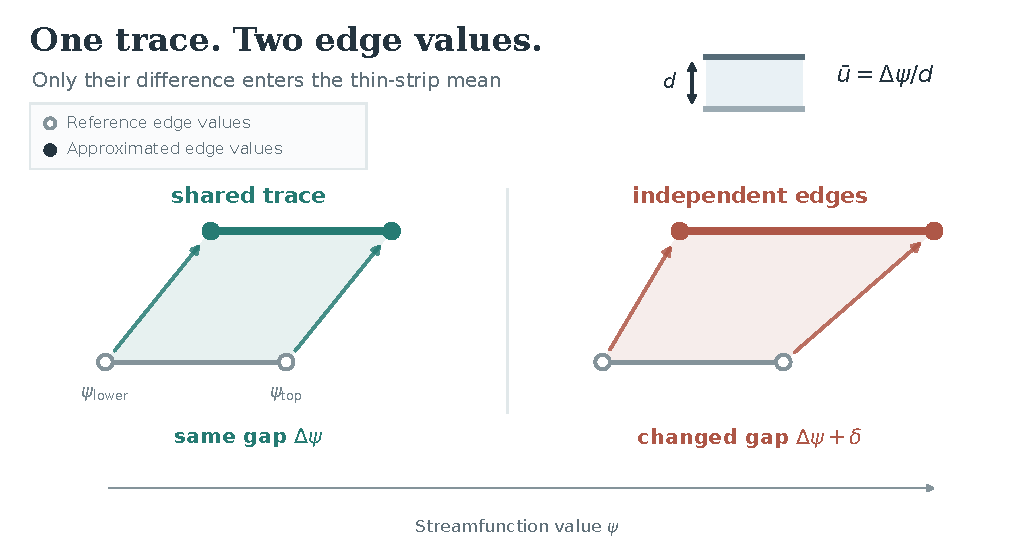
\includegraphics[width=\linewidth]{figures/method_principle.pdf}
\caption{A shared trace preserves the difference of two edge values.
The connected markers represent the two edge-averaged streamfunction
values; horizontal position denotes value, while vertical separation
distinguishes the reference and perturbed representations.
Equal shifts translate the segment without changing its length;
independent shifts deform it, introducing a mismatch divided by the
small strip thickness $d$. The matched extension constructs both averages
from the same physical trace, cancelling its common error before division.
Errors in the normal derivatives remain, as quantified by
\eqref{eq:matched-strip-bound}. The diagram illustrates the unblended
flat-strip construction; the Cartesian blend is described in the text.}
\label{fig:method-principle}
\end{figure}

\subsection{MAC flux identity}
Using streamfunction values at Cartesian vertices, the normal face averages
can also be defined by endpoint differences. With consistent indexing,
\begin{equation}
 U_{i,j+1/2}=\frac{\psi_{i,j+1}-\psi_{i,j}}{h},\qquad
 W_{i+1/2,j}=-\frac{\psi_{i+1,j}-\psi_{i,j}}{h}.
\end{equation}
Their Cartesian cell divergence vanishes algebraically because the mixed
differences commute. These face quantities are retained separately from the
liquid moments. The identity does not include the receiver's open-face
fractions, embedded boundary fluxes, or its interpolation on loading.

\subsection{Optional projection to a mixture velocity}
A one-fluid receiver stores one velocity per cell, whereas the preceding
construction supplies a liquid-phase mean. If a gas-phase mean
$\overline{\boldsymbol u}_{g,K}$ is also prescribed, a density-weighted
projection is
\begin{equation}
 \boldsymbol v_K^{\rm mix}=
 \frac{\rho_\ell q_K\overline{\boldsymbol u}_{\ell,K}
       +\rho_g(c_{s,K}-q_K)\overline{\boldsymbol u}_{g,K}}
      {\rho_\ell q_K+\rho_g(c_{s,K}-q_K)}
 \quad(c_{s,K}>0).
 \label{eq:mixture-projection}
\end{equation}
Multiplying by the cell fluid mass gives the sum of the represented
phase momenta. Equivalently, this is the constant cell vector that minimises
the density-weighted squared discrepancy from the two phase fields.
This standard projection is distinct from assigning the liquid mean to
every liquid-containing cell. In the tested surface strip with
$q_K=0.0005$ and $c_{s,K}=1$, gas supplies about 70\% of the cell mass,
despite its small density; the two assignments can therefore differ
appreciably. The phase-moment closure established above applies before
this projection. The mixed vector must not subsequently be counted as a
liquid-phase mean when checking that identity.

We test this projection as an alternative receiver assignment, using a
common prescribed gas phase for every transfer variant. Its usefulness
depends on the receiver's discrete variable and gas initialisation; the
formula alone does not prove compatibility with an arbitrary VOF solver.
The original native comparisons retain their liquid-mean assignment, and
the independent two-fluid test compares the two assignments explicitly.

\section{Matching the receiving geometry}
The receiver is Aphros, an incompressible multiphase finite-volume solver
with embedded boundaries and geometric VOF transport~\citep{karnakov,aphros}. Its
embedded geometry is reconstructed from nodal signed-distance data.
Preparing fractions from an independently clipped bed polygon can produce
$q_K>c_{s,K}^{\mathrm{native}}$. A loading operation that clips the liquid
fraction to the available fluid volume then loses liquid even when the
offline volume is exact.

The preparation procedure reproduces the receiver's nodal edge crossings,
constructs the corresponding bed, and integrates the liquid fractions and
moments on that geometry. A small uniform surface-height adjustment
reconciles the source volume with the polygonal volume; it is a
geometric adjustment, not a redistribution of liquid among arbitrary cells.
Its magnitude is measured for each prepared state. The embedded-bed
reconstruction requires a resolved single-valued periodic graph and supported
cell crossing topology; degenerate configurations are rejected.

After loading, the receiver applies its own pressure projection. Native
embedded-volume flux divergence is measured independently of the offline
MAC identity. The measurement protocol distinguishes input velocity, loaded
velocity, and projected velocity; pressure-system residuals and embedded
flux divergence are not interchangeable acceptance criteria.

The receiver uses the projection solver with AMGX for the symmetric
pressure system. In the numerical units of the supplied state, the liquid
and gas densities are 1 and 0.00117647, their dynamic viscosities are
$2.5\times10^{-5}$ and $4.88764\times10^{-7}$, surface tension is 0.001,
and gravity is $(0,-1)$. For the fixed overturning-state startup, the baseline controls are CFL
0.05 and maximum time step $6.25\times10^{-4}$; the time-step variations
are specified in Appendix~\ref{app:time-step}. The main smooth-wave
continuations use the separate settings specified in
Section~\ref{sec:native-protocol}; neither test is calibrated to a
laboratory wave case.

\paragraph{Transfer procedure.}
The following steps specify how the geometry, streamfunction, and receiver
data are coupled. Steps 1--3 and 5 apply to the general polygonal operator;
step 4 is used only for the flat-strip Matched variant.
\begin{enumerate}
\item Reconstruct the receiver's embedded bed from its nodal signed-distance
data, clip the liquid polygons on that geometry, and check source boundary
flux compatibility.
\item Integrate the source normal-velocity trace to obtain the boundary
streamfunction and fix the relative boundary constant from source transport.
Solve the liquid harmonic Dirichlet problem and complete the vertices needed
by the liquid polygons.
\item Give each shared polygon edge one scalar streamfunction integral,
with opposite orientation in its two cells.
\item On flat upper strips, use the same cubic boundary trace on the physical
edge and in $J(d)$; blend its neighbouring Cartesian edge through
\eqref{eq:matched-blend}. Both adjacent cells use this shared edge integral.
\item Sum the oriented edge moments using~\eqref{eq:green}, divide by
liquid area, and supply the liquid means and matched fractions to the receiver. If
the receiver instead requires a mixture velocity, use the separately
defined projection~\eqref{eq:mixture-projection} with prescribed gas means.
\end{enumerate}

\section{Numerical experiments}
\subsection{Error measures and test cases}
For a reference liquid volume $V_*$ and momentum $\boldsymbol M_*$, report
\begin{equation}
 e_V=\frac{|\sum_Kq_Kh^2-V_*|}{V_*},\qquad
 e_M=\frac{\|\boldsymbol M_h-\boldsymbol M_*\|_2}{\|\boldsymbol M_*\|_2}.
\end{equation}
The relative momentum error is used only for a nonzero target. The analytic
periodic tests have zero net momentum and retain absolute moment defects
instead of dividing by their roundoff-sized target.
For phase means on a selected set $\mathcal S$, an explicitly
phase-volume-weighted relative norm can be defined by
\begin{equation}
 e_{\ell,2}^2=
 \frac{\sum_{K\in\mathcal S}q_Kh^2
       \|\overline{\boldsymbol u}_{\ell,K}-\overline{\boldsymbol u}_{*,K}\|_2^2}
      {\sum_{K\in\mathcal S}q_Kh^2\|\overline{\boldsymbol u}_{*,K}\|_2^2}.
 \label{eq:l2}
\end{equation}
Probe and sampled-reference results below use their stated norms, which
may differ from~\eqref{eq:l2}. Sources for the experimental code and data
are given in \hyperref[sec:data-code]{Data and code availability}.

\subsection{Native propagation of transfer error}\label{sec:native-protocol}
A separate smooth-wave benchmark measures the subsequent influence of
initial transfer error against a computable reference input. The periodic
length is 64, the flat receiver bed is at $z_b=0.53000001$, and the initially
flat free surface is at $z_s=1.5000625$. We use grids $512\times32$,
$1024\times64$ and $2048\times128$, with the same physical geometry. Their
upper liquid-row fractions are respectively 0.0005, 0.001 and 0.002. The prescribed initial potential is
\begin{equation}
 \phi(x,z)=A\cos(kx)\frac{\cosh(k(z-z_b))}{\cosh(kD)},\qquad
 A=0.02,\quad k=2\pi\,16/64,\quad D=z_s-z_b.
\end{equation}
There is no background current. The reference input consists of exact
liquid-cell means of $\nabla\phi$, integrated analytically over the rectangular
liquid portions. An independent eight-point tensor Gaussian integration
agrees with these means to $1.86\times10^{-14}$ in relative liquid-weighted norm.

The principal comparison uses Matched (M), Bilinear (B) and exact initial
means on one corrected receiver build. The boundary source has 512 nodes;
trace factors 8, 8 and 16 give trace/grid-spacing ratios 0.125, 0.25 and
0.25. The first two levels reproduce the previous input policy, while the
third retains the second level's ratio. Earlier Linear (L) and time-step
comparisons are retained in Appendix~\ref{app:general-tests}.
Their geometry, gas velocities, physical coefficients and receiver settings
are identical, and the receiver reconstructs its initial face fluxes from
each branch's own cell velocities. Zero target momentum is checked with an
absolute tolerance $10^{-6}$, rather than an ill-defined relative error.
The physical coefficients are those listed above. The nominal inviscid
capillary--gravity time scale, neglecting gas density in the dispersion
relation \citep{fitzpatrick}, is
$T=2\pi/\sqrt{(gk+\sigma k^3/\rho_\ell)\tanh(kD)}=5.25072$;
it is used only to specify the common endpoint $t=0.1T=0.52507177$.
The reference branch is a numerical continuation from exact initial means,
not an exact later-time two-phase solution.

With $R$ denoting the exact-input reference and $A$ a tested initialisation,
the primary global error is
\begin{equation}
 E_u^2(t)=\frac{\sum_Kq_K^R(t)\|\boldsymbol u_K^A(t)-\boldsymbol u_K^R(t)\|_2^2}
                    {\sum_Kq_K^R(t)\|\boldsymbol u_K^R(t)\|_2^2}.
 \label{eq:dynamic-error}
\end{equation}
For $X\in\{M,B\}$, let $f_{ij}^X$ and $c_{s,ij}^X$ be the output liquid
and non-solid fractions in horizontal column $i$ and vertical cell $j$.
The VOF error is $\|f^X-f^R\|_2/\|f^R\|_2$. The column depth and its
wave-normalised error are
\begin{equation}
 H_i^X(t)=h\sum_j f_{ij}^X(t)c_{s,ij}^X(t),\qquad
 E_H^X(t)=\frac{\|H^X(t)-H^R(t)\|_2}
 {\|H^R(t)-\langle H^R(t)\rangle\|_2}.
 \label{eq:dynamic-depth-error}
\end{equation}
Here $R$ is the same-grid numerical continuation from exact initial means,
and the denominator is the instantaneous wave component of that trajectory;
$E_H$ is undefined for its initially flat surface. The independent physical
test below instead uses a fixed analytic wave-amplitude denominator. The
primary runs use $\Delta t_{\max}=0.0025$ and
CFL 0.1. The earlier half-step control uses 0.00125 and CFL 0.05.

\section{Results}
The main comparisons concern the Matched extension on flat surface strips.
Tests of the general polygonal construction and earlier transfer
variants are reported in Appendix~\ref{app:general-tests}.

\subsection{Analytic initial-field tests of the Matched extension}
We evaluate the extension in~\eqref{eq:matched-jet} in 15 cases:
manufactured mode-4 fields (F4, defined by
Eq.~\eqref{eq:manufactured-f4} in the Appendix) at $n_x=128,256$, with upper-strip liquid
fractions $10^{-5},10^{-3},10^{-2},10^{-1}$; mode-16 wave fields at
$n_x=512$ with fractions $0.0005,0.001,0.01,0.1$; and mode-16 fields at
$n_x=1024$ with fractions $0.001,0.01,0.1$. Closed-form phase-cell means
provide the reference. Source data, geometry and the comparison cases
are fixed within each comparison. No analytic interior field is used by
the matched operator.

Hermite (H) changes only the physical trace, while Matched (M) also uses
it on the neighbouring Cartesian edge. The two cases in
Table~\ref{tab:lhm-ablation} isolate this difference. A higher-order
physical trace alone does not reproduce the improvement from matching the
two edge representations.

\begin{table}[htbp]\centering\small
\caption{Thin upper-row relative velocity error against analytic phase-cell
means. L uses a linear physical trace, H a cubic Hermite physical trace,
and M matches that trace across the neighbouring Cartesian edge.
The two rows use the same source data and geometry within each case.}
\label{tab:lhm-ablation}
\begin{tabular}{@{}lrrr@{}}\toprule
Case & Linear (L) & Hermite (H) & Matched (M)\\\midrule
F4, $n_x=128$, $q_{\rm top}=0.001$ & 0.03757 & 0.08046 & $9.07\times10^{-6}$\\
W16, $n_x=512$, $q_{\rm top}=0.0005$ & 0.18570 & 0.15833 & $3.70\times10^{-5}$\\
\bottomrule\end{tabular}
\end{table}

M reduces both the top-row error and the all-liquid, volume-weighted error
in all 15 cases relative to L and H. It also improves the global error
relative to B in all 15 cases,
by factors 2.71--12.60 (Table~\ref{tab:matched-extension}). Its maximum
top-row relative error over this matrix is $5.16\times10^{-5}$; the maximum
absolute moment-closure defect is $2.61\times10^{-15}$.
For the original wave geometries, the global initial error decreases from
0.002987 to 0.001420 at $512$ columns and from 0.004700 to 0.0003538 at
$1024$ columns. The remaining global error includes the interior and bed
cells, which the surface extension does not directly correct. These
measurements concern initial phase means; the evolved-field comparisons
follow below.

\begin{table}[htbp]
\centering\small
\caption{Complete declared initial-field comparison for the matched boundary extension. Errors are liquid-volume-weighted relative velocity norms over all liquid cells. M denotes the manufactured mode-4 family; W denotes the mode-16 wave family. The control uses the same computed streamfunction. These are initial-field errors, not evolved-wave errors.}\label{tab:matched-extension}
\begin{tabular}{@{}lrrllll@{}}\toprule
Family & $n_x$ & $q_{\rm top}$ & Linear & Matched & Control & Gain\\\midrule
M & 128 & 1e-05 & 7.049e-03 & 1.475e-03 & 3.993e-03 & 2.71\\
M & 128 & 0.001 & 1.678e-03 & 1.474e-03 & 4.184e-03 & 2.84\\
M & 128 & 0.01 & 1.553e-03 & 1.462e-03 & 5.606e-03 & 3.83\\
M & 128 & 0.1 & 1.603e-03 & 1.356e-03 & 1.202e-02 & 8.87\\
M & 256 & 1e-05 & 1.693e-03 & 3.526e-04 & 9.936e-04 & 2.82\\
M & 256 & 0.001 & 3.870e-04 & 3.524e-04 & 1.092e-03 & 3.10\\
M & 256 & 0.01 & 3.548e-04 & 3.507e-04 & 1.738e-03 & 4.96\\
M & 256 & 0.1 & 3.614e-04 & 3.352e-04 & 4.223e-03 & 12.60\\
W & 512 & 0.0005 & 2.987e-03 & 1.420e-03 & 4.087e-03 & 2.88\\
W & 512 & 0.001 & 2.324e-03 & 1.420e-03 & 4.183e-03 & 2.95\\
W & 512 & 0.01 & 1.503e-03 & 1.407e-03 & 5.612e-03 & 3.99\\
W & 512 & 0.1 & 1.470e-03 & 1.298e-03 & 1.205e-02 & 9.28\\
W & 1024 & 0.001 & 4.700e-03 & 3.538e-04 & 1.090e-03 & 3.08\\
W & 1024 & 0.01 & 1.495e-03 & 3.520e-04 & 1.735e-03 & 4.93\\
W & 1024 & 0.1 & 5.098e-04 & 3.361e-04 & 4.218e-03 & 12.55\\
\bottomrule\end{tabular}
\end{table}


A further six cases use mode~7 at
$n_x=512,1024$ and $q_{\rm top}=0.3,0.7,0.99$ with the same operator.
The global error remains lower than B in all six cases, by factors
3.73--32.07. These larger
fractions also exercise the transition back to Cartesian integration.
At $q_{\rm top}=0.99$ the M and H top-row errors
nearly coincide, with the M value about 0.2\% larger; the matched
extension therefore is not uniformly superior to that ablation at all
fractions. Its moment-closure defect remains below $5.32\times10^{-17}$.

Table~\ref{tab:joint-refinement} tests the final M operator on three grids
while refining the boundary trace with the receiver: its spacing is $h/8$
throughout. The global velocity error decreases from $1.4203\times10^{-3}$
to $3.5378\times10^{-4}$ and $8.0414\times10^{-5}$, with observed orders
2.005 and 2.137. B uses the same computed streamfunction and has larger
errors on all three grids. These are transfer-refinement results for a
fixed boundary source state; they do not establish convergence of the
upstream boundary solver. The cut-cell errors and maximum vector errors
are retained with the global norms in the accompanying data.
\begin{table}[tbp]\centering\small
\caption{Initial liquid-volume-weighted velocity error under joint grid and trace refinement (W16). The refined trace spacing is $h/8$ on each grid. Orders compare successive rows; the source boundary state has 512 nodes throughout.}\label{tab:joint-refinement}
\begin{tabular}{@{}rrrrrrr@{}}\toprule
$n_x$ & Trace points & $E_M$ & Order & $E_B$ & Order & $E_B/E_M$\\\midrule
512 & 4096 & 1.4203e-03 & --- & 4.0869e-03 & --- & 2.88\\
1024 & 8192 & 3.5378e-04 & 2.005 & 1.0898e-03 & 1.907 & 3.08\\
2048 & 16384 & 8.0414e-05 & 2.137 & 3.3498e-04 & 1.702 & 4.17\\
\bottomrule\end{tabular}
\end{table}


\subsection{Propagation of transfer error}\label{sec:dynamic-results}
The three-grid comparison uses the same corrected receiver executable and
library for all nine M, B and exact-input branches. Common geometry, gas
velocities, physical coefficients and time-step controls isolate the
initial transfer. The receiver reconstructs its face fluxes from each
branch's cell velocities; the common supplied face arrays are not imposed
as runtime fluxes.

Table~\ref{tab:audited-dynamics} reports the errors at $t=0.1T$.
M reduces the global velocity discrepancy by factors of 7.88, 9.80 and
17.81 on the three grids. The corresponding surface-profile reductions
are 65.0, 73.8 and 102.4. Both improvements hold at every recorded
nonzero time (Fig.~\ref{fig:audited-dynamics}). The maximum recorded
relative liquid-mass discrepancy is $7.15\times10^{-13}$, and the maximum
post-start flux divergence is $6.99\times10^{-14}$.

The M endpoint velocity errors are $1.7585\times10^{-3}$,
$4.3460\times10^{-4}$ and $9.8215\times10^{-5}$.
Their two-level observed orders are 2.017 and 2.146. This native series
uses the trace policy specified in Section~\ref{sec:native-protocol};
the fixed trace/grid-ratio initial test is reported separately in
Table~\ref{tab:joint-refinement}. The earlier full- and half-step
comparisons are retained in Appendix~\ref{app:old-matched}; the three-grid
results here establish the transfer advantage on one documented corrected
receiver build.
\begin{table}[tbp]\centering\small
\caption{Propagated transfer error at $t=0.1T$ on the common corrected receiver build. Each reference trajectory starts from exact cell means on the same grid. $E_u$ is the liquid-weighted velocity error and $E_H$ the wave-normalised column-depth discrepancy; $R=E_B/E_M$.}\label{tab:audited-dynamics}
\begin{tabular}{@{}rrrrrrr@{}}\toprule
$n_x$ & $E_u^M$ & $E_u^B$ & $R_u$ & $E_H^M$ & $E_H^B$ & $R_H$\\\midrule
512 & 1.7585e-03 & 1.3861e-02 & 7.88 & 3.9263e-05 & 2.5528e-03 & 65.02\\
1024 & 4.3460e-04 & 4.2597e-03 & 9.80 & 7.3386e-06 & 5.4177e-04 & 73.83\\
2048 & 9.8215e-05 & 1.7489e-03 & 17.81 & 1.6265e-06 & 1.6651e-04 & 102.38\\
\bottomrule\end{tabular}
\end{table}


\begin{figure}[htbp]\centering
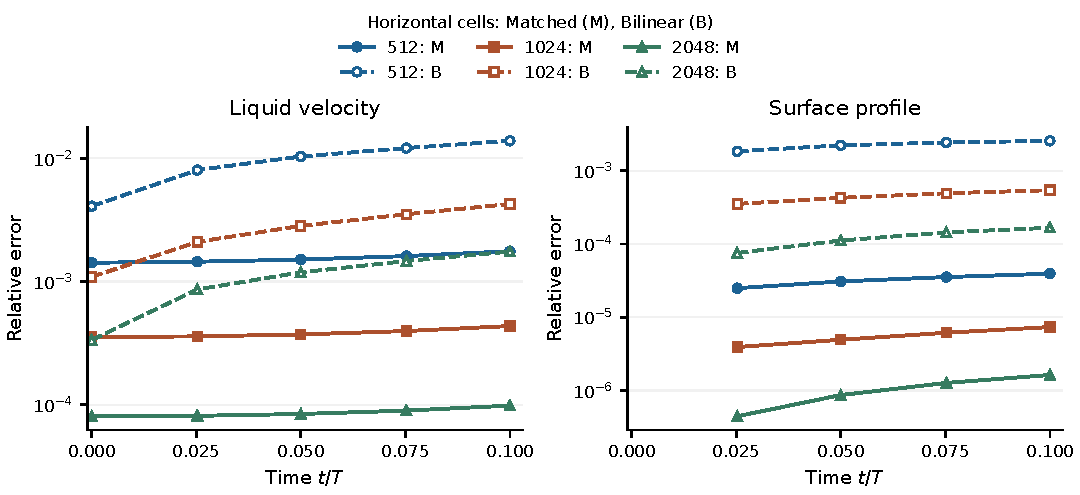
\includegraphics[width=\linewidth]{figures/audited_native_dynamics.pdf}
\caption{Propagated transfer error on three grids using the common corrected
receiver build and $\Delta t_{\max}=0.0025$. Each curve is compared with the
exact-input numerical trajectory on its own grid. Filled markers and solid
lines denote M; open markers and dashed lines denote B. Surface error is
shown at every nonzero output time; its normalisation is undefined for the
initially flat profile.}\label{fig:audited-dynamics}
\end{figure}

\subsection{Independent small-amplitude two-fluid wave}
An additional benchmark compares the evolved column depth with an
independent linear two-fluid capillary--gravity wave. It uses the same
physical geometry and density ratio, but zero viscosity, a slip bottom
and a pressure-release upper boundary. The assignment comparison uses
$512\times32$ cells; its spatial check adds $1024\times64$ cells.
Let $D_\ell=z_s-z_b$ and
$D_g=4-z_s$, with the upper boundary at $z=4$. The linear frequency
and surface amplitude for initial liquid potential
$A\cos(kx)\cosh(k(z-z_b))/\cosh(kD_\ell)$ are
\begin{equation}
 \omega^2=\frac{(\rho_\ell-\rho_g)gk+\sigma k^3}
 {\rho_\ell\coth(kD_\ell)+\rho_g\tanh(kD_g)},\qquad
 B=\frac{Ak\tanh(kD_\ell)}{\omega}.
\end{equation}
The corresponding initial gas potential is
$-A\tanh(kD_\ell)\sinh(k(4-z))\cos(kx)/\cosh(kD_g)$.
It satisfies the linear kinematic condition at the interface and the
pressure-release condition at the top. We check the boundary-equation
residuals and evaluate the phase-cell means independently by quadrature.
The reference column depth averaged over a horizontal cell is
\begin{equation}
 H_i^{\rm lin}(t)=D_\ell+B\sin(\omega t)
 \operatorname{sinc}(kh/2)\cos(kx_i),\qquad
 \operatorname{sinc}(s)=\sin(s)/s.
\end{equation}
Here the depth-error RMS is normalised by the fixed quantity
$B\operatorname{sinc}(kh/2)/\sqrt{2}$; this differs from the instantaneous
numerical-reference normalisation in Fig.~\ref{fig:audited-dynamics}.
The endpoint is $t=0.1(2\pi/\omega)=0.52566088$ and
$\Delta t_{\max}=0.00125$.

A zero-amplitude control exposed an undefined zero-displacement operation
in the receiver's two-dimensional geometric VOF flux routine. Returning
zero transported volume for zero displacement prevents the 0.403\% first-step
liquid loss of the unmodified build. The corrected rest control preserves
mass and has endpoint depth-error RMS $1.11\times10^{-16}$.
The physical-reference tests and the three-grid propagation comparison
use this same corrected build. The earlier unmodified-runtime comparisons
are retained in Appendix~\ref{app:old-matched}.

With exact initial phase means, $A=2\times10^{-5}$ gives normalised
depth error 0.03533528 at the endpoint; $A=10^{-5}$ gives 0.03533601.
The absolute errors are $5.96216\times10^{-7}$ and
$2.98114\times10^{-7}$. Their near-linear amplitude scaling and the
separate rest control support comparison with the linear reference at
these amplitudes. This reference tests a smooth inviscid wave, not a
nonlinear breaking-wave solution.

For the transfer comparison, M and B
liquid inputs are scaled by $10^{-3}$ to $A=2\times10^{-5}$, without
retuning the operator. The corresponding scaled exact liquid field agrees
with the independently integrated phase means within
$5.88\times10^{-17}$ in maximum absolute velocity. Geometry and dry/gas
cell velocities are identical across the three branches, and each branch
uses the same native flux-reconstruction procedure.
Table~\ref{tab:physical-wave} reports the complete nonzero-time comparison.
At the endpoint, M reduces the normalised physical depth
error from 0.03718424 to 0.03535843, a 4.91\% reduction. It improves this
metric at every recorded nonzero time, with reductions from 4.91\% to
13.01\% over the four samples.

The discrepancy from the exact-input numerical trajectory is much smaller:
its normalised depth RMS is $2.31536\times10^{-5}$ for M
and $1.84896\times10^{-3}$ for B, a factor of 79.86.
Their global liquid-weighted velocity discrepancies are 0.00168245 and
0.01070309, a factor of 6.36. The moderate 4.91\% improvement against
the analytic wave is therefore compatible with a much larger reduction
of the transfer contribution: the exact-input receiver already has a
physical depth error of 0.03533528. Each of these three branches preserves liquid mass;
the maximum measured post-start flux divergence is below $10^{-15}$.
The three branches share endpoint times, geometry, and receiver settings.
\begin{table}[htbp]\centering\small
\caption{Depth-error RMS against the independent linear two-fluid wave,
normalised by the fixed analytic wave-amplitude RMS. All recorded
nonzero times are included. The last column is the relative reduction
from the practical control to the matched transfer.}
\label{tab:physical-wave}
\begin{tabular}{rrrrr}\toprule
$t$ & Exact input & Matched & Practical & Reduction (\%)\\\midrule
0.13125 & 0.00248271 & 0.00248760 & 0.00285971 & 13.01\\
0.26250 & 0.00811344 & 0.00812471 & 0.00900079 & 9.73\\
0.39375 & 0.01821401 & 0.01823153 & 0.01960601 & 7.01\\
0.52566 & 0.03533528 & 0.03535843 & 0.03718424 & 4.91\\
\bottomrule\end{tabular}
\end{table}


The alternative assignment in~\eqref{eq:mixture-projection} uses the same
wave protocol. With exact phase means it reduces
the endpoint physical depth error from 0.03533528 to 0.01775465.
At half amplitude the corresponding error is 0.01775438, again preserving
the linear scaling, and both runs preserve liquid mass. This experiment
supports the density-weighted assignment for this receiver and state;
it does not establish a universal VOF velocity contract.

The complete factorial comparison retains all six combinations of phase
reconstruction and receiver assignment (Table~\ref{tab:mixture-factorial}).
With density-weighted projection, M gives endpoint physical
depth error 0.01777826, compared with 0.01881090 for B:
a 5.49\% reduction under identical receiver assignment.
The combined M-plus-mixture construction reduces the error from
the original B liquid-mean assignment, 0.03718424, by 52.19\%
(a factor of 2.092). The latter improvement includes both changes and
must not be attributed to the boundary extension alone.

The combined construction improves on the original B assignment
at every recorded nonzero time. Within the mixture assignment, however,
the B control has the smaller physical error at the first sample
($t=0.13125$: 0.00016171 versus 0.00040606); M is better
at the three later samples. Lower initial transfer error therefore need
not minimise total physical error at each individual time.
Against the exact-mixture-input numerical trajectory, the endpoint depth
discrepancies are $2.36173\times10^{-5}$ and $1.05626\times10^{-3}$
for M and B, respectively. These transfer-only
discrepancies are distinct from the physical errors in the table.
The mixed-cell inputs use separately integrated gas-phase means and satisfy
the density-weighted formula to roundoff.
\begin{table}[htbp]\centering\small
\caption{Factorial comparison at $0.1T$ against the independent
linear two-fluid wave: normalised physical depth-error RMS.
Each column uses the same phase reconstruction under both
receiver assignments; geometry, gas phase and runtime are common.}
\label{tab:mixture-factorial}
\begin{tabular}{lrrr}\toprule
Receiver assignment & Exact phase data & Matched & Practical\\\midrule
Liquid mean in wet cells & 0.03533528 & 0.03535843 & 0.03718424\\
Density-weighted mixture & 0.01775465 & 0.01777826 & 0.01881090\\
\bottomrule\end{tabular}
\end{table}


The spatial check repeats M, B and exact-input runs with mixture assignment
on $512\times32$ and $1024\times64$ cells, holding the amplitude, physical
geometry, boundary conditions and time-step limit fixed.
Table~\ref{tab:physical-refinement} includes every recorded nonzero time.
The coarse-grid endpoint reproduces the 5.49\% reduction. On the finer
grid, M reduces physical depth error from 0.00985114 to 0.00957410,
a 2.81\% reduction, and improves on B at all four nonzero samples.
The M endpoint error decreases by a factor of 1.857 under refinement;
the exact-input error decreases from 0.01775465 to 0.00957065.
The remaining physical error is therefore close to that of the exact-input
receiver, even though the transfer contribution is much smaller with M.
All six runs preserve liquid mass at output precision, with maximum recorded
post-start flux divergence $5.51\times10^{-15}$.
\begin{table}[tbp]\centering\small
\caption{Physical column-depth error against the cell-averaged linear two-fluid wave, with density-weighted receiver assignment held fixed. Errors use the fixed linear-wave RMS amplitude. Every recorded nonzero time is included; the reduction is $100(1-E_M/E_B)$.}\label{tab:physical-refinement}
\begin{tabular}{@{}rrrrrr@{}}\toprule
$n_x$ & $t$ & Exact input & Matched (M) & Bilinear (B) & Reduction (\%)\\\midrule
512 & 0.13125 & 0.00041102 & 0.00040606 & 0.00016171 & -151.10\\
512 & 0.26250 & 0.00026377 & 0.00027524 & 0.00079983 & 65.59\\
512 & 0.39375 & 0.00529807 & 0.00531594 & 0.00610920 & 12.98\\
512 & 0.52566 & 0.01775465 & 0.01777826 & 0.01881090 & 5.49\\
\midrule
1024 & 0.13125 & 0.00006724 & 0.00006795 & 0.00012428 & 45.33\\
1024 & 0.26250 & 0.00075300 & 0.00075460 & 0.00088189 & 14.43\\
1024 & 0.39375 & 0.00337341 & 0.00337593 & 0.00357862 & 5.66\\
1024 & 0.52566 & 0.00957065 & 0.00957410 & 0.00985114 & 2.81\\
\bottomrule\end{tabular}
\end{table}


\subsection{Computational cost of the transfer}
Table~\ref{tab:transfer-cost} isolates the in-memory Matched transfer on
an Intel Core Ultra 7 155H CPU under Windows 11, using Python 3.13.3,
NumPy 2.3.5, SciPy 1.17.1 and Shapely 2.1.2. The trace factors are 8 and
16 on the two grids. Each timing uses three repetitions after one warm-up;
the output velocity arrays are byte-identical across repetitions.
The measured transfer includes geometry, the liquid solve, gas continuation,
cell moments and Cartesian face-velocity preparation, but excludes serialization, checkpoints
and subsequent flow evolution. Boundary-trace preparation is timed
separately. Liquid-cell moment construction accounts for approximately
half of the median transfer time in this implementation. The remaining
in-memory category is the total transfer time minus the separately timed
assembly, liquid solve, gas continuation and cell moments. It includes
liquid-aperture construction, exterior liquid-support continuation,
Cartesian face velocities and divergence diagnostics. These measurements
describe the current CPU code, rather than a GPU speedup or an asymptotic
complexity estimate.
\begin{table}[tbp]\centering\small
\caption{CPU transfer cost in seconds: median [minimum, maximum] over three repetitions after one warm-up. Stages exclude file output, checkpoints and CFD evolution. Stage medians need not sum to the median total.}\label{tab:transfer-cost}
\begin{tabular}{@{}lrr@{}}\toprule
Stage & $512\times32$ & $1024\times64$\\\midrule
Boundary trace & 0.0212 [0.0167, 0.0225] & 0.0450 [0.0409, 0.0483]\\
Geometry and harmonic-system assembly & 0.1028 [0.1020, 0.1114] & 0.4387 [0.3556, 0.4480]\\
Liquid harmonic solve & 0.0018 [0.0017, 0.0018] & 0.1013 [0.0539, 0.1332]\\
Gas continuation & 0.0144 [0.0085, 0.0192] & 0.3019 [0.2840, 0.3689]\\
Liquid-cell moments & 1.9355 [1.8201, 2.2680] & 12.3647 [10.1513, 12.4287]\\
Remaining in-memory operations & 1.8810 [1.7302, 3.2785] & 11.1201 [10.4661, 12.9108]\\
Transfer total, excluding trace & 3.8285 [3.7779, 5.6702] & 23.5884 [22.1545, 26.1844]\\
\bottomrule\end{tabular}
\end{table}


\section{Discussion and limitations}
The main gain comes from coupling two edge representations. Raising the
physical-trace order alone does not remove their mismatch in a thin strip.
The bound~\eqref{eq:matched-strip-bound} explains cancellation of the
common trace error, while the derivative errors and the Cartesian blend
remain. It gives a uniform refinement rate only under the stated bounds
on derivative sampling and $I_C-J(d)$; those bounds have not been proved
for the coupled harmonic solve. The observed refinement rates therefore complement the local mechanism
rather than establish an unconditional convergence theorem.

The smooth-wave trajectories started from exact cell means isolate the
effect of initial transfer under a common numerical receiver. Their error
against each other should not be read as physical error. The independent
linear two-fluid wave supplies a physical reference and shows a smaller
gain. Receiver velocity assignment also matters: the 52.19\% combined
reduction on the coarse grid includes both Matched transfer and the standard
mixture projection, whereas the 2.81--5.49\% comparisons hold assignment
fixed. With mixture assignment, B is better at the first recorded nonzero
time on the coarse grid; M is better at the three later samples and all
four fine-grid samples. Cross-step comparisons can reverse
the ranking because temporal and transfer errors interact
(Appendix~\ref{app:general-tests}).

The polygonal moment construction has a wider geometric scope than the
flat-strip extension, but its discrete closure does not ensure local
accuracy. The earlier Linear variant improves selected native bed-cut
cells over B, while an exact-field centroid sample is more accurate in
the nine pooled flat cut-cell tests (Appendix~\ref{app:general-tests}).
The fixed overturning state has surface-height span 0.77104 and a
non-monotone horizontal parametrisation. M rejects this geometry; its
transfer and native startup test only the general polygonal construction.
The fixed-state continuation has no independent evolved reference.

The tests use two-dimensional periodic geometry and zero background
current. The local estimate covers the horizontal mean in flat strips;
the independent BIE sample covers 12 selected bed-cut cells. The smooth
native runs are short, and neither the upstream wave formation nor a
complete breaking-wave trajectory has been shown to converge in space
and time. An extension to overturning boundaries would require a
curved-boundary construction and its own accuracy analysis.

\section{Conclusions}
For thin strips beneath a flat surface, Matched transfer uses one physical
trace on both sides of the edge difference. The common trace error cancels
before division by the small strip thickness. The bound for the implemented
blend identifies the remaining derivative and Cartesian-edge errors.
Across 21 analytic initial-field tests, M lowers global velocity error
relative to B. A separate three-grid initial test gives observed orders
2.005 and 2.137 under joint trace/grid refinement. On a common corrected
receiver build, the three-grid continuations reduce propagated velocity
error by factors of 7.88--17.81 and surface-profile error by 65.0--102.4
against same-grid numerical trajectories started from exact cell means.

Against an independent linear two-fluid wave, M lowers endpoint physical
surface-profile error by 5.49\% and 2.81\% on the two grids when mixture
assignment is held fixed. On the coarse grid, combining M with that
standard assignment lowers the error by 52.19\% relative to the original
practical B input with liquid-mean assignment;
this larger reduction includes both changes. The more general polygonal
construction preserves discrete liquid moments by shared-edge cancellation,
and receiver-matched geometry avoids liquid loss on loading. The flat-strip
accuracy estimate does not apply to overturning surfaces, and these short
continuations do not validate a complete breaking-wave trajectory.

\section*{Data and code availability}\phantomsection\label{sec:data-code}
The original code, benchmark inputs and numerical evidence are archived
as v0.31.0~\citep{baturin-transfer}. The additional refinement, dynamic,
physical-reference and cost experiments are archived in
v0.32.0~\citep{baturin-followup}. It includes the input and output fields,
analysis scripts, transfer sources, corrected receiver source and patch,
build records, and runtime configuration hashes used in the principal
comparisons. Its verifier recomputes the three main numerical audits from
the archived input and output fields, without rerunning the CFD solver.
The archived sources, build records, runtime hashes and campaign commands
support a separate full rerun from the initial state with the required
receiver toolchain. Historical source-provenance limits remain documented
with the original archive; its DOI does not identify the later experiments.

\section*{Funding}
The work received no external funding.
\section*{Conflict of interest}
The author declares no competing interests.
\section*{Additional information}
\ifdefined\BlindReview
The manuscript has one author.
\else
Saveliy Baturin is the sole author.
\fi
The work is original and has not been submitted to another journal.

\clearpage
\appendix
\section{General polygonal transfer and earlier variants}\label{app:general-tests}
These tests document the base polygonal operator, trace resolution,
and receiver sensitivity. They do not use the flat-strip Matched
extension on the overturning geometry.

The fixed wave state has 2304 nodes on each boundary and comes from a
refined boundary solve on a fixed geometry. The convergence of its upstream
nonlinear BIE trajectory was not assessed here.
Its target liquid volume is $40.52627859944759$. The grids are
$1024\times64$, $2048\times128$, and $4096\times256$ for $L=64$.
The finest spacing is $h=0.015625$. Refining these receiver grids with the
same source tests the transfer and receiver sensitivity, not the convergence
of the upstream time-dependent BIE solution.
Figure~\ref{fig:geometry} shows the source boundary geometry.

\begin{figure}[hbp]\centering
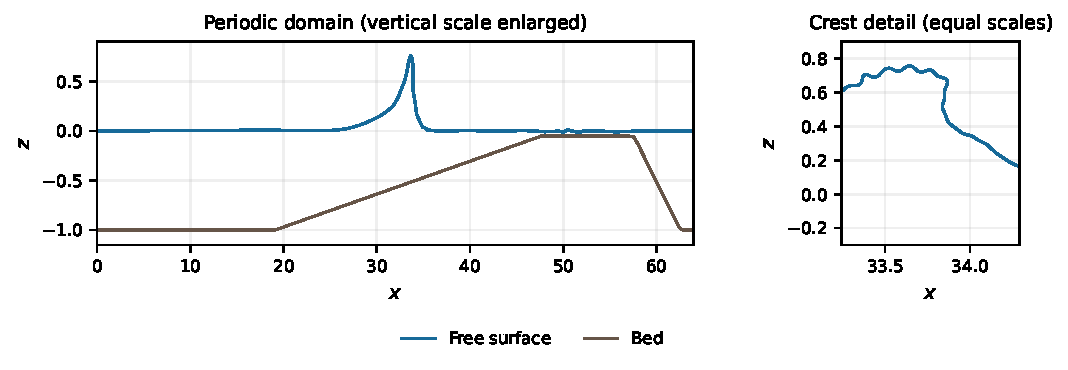
\includegraphics[width=\linewidth]{figures/fixed_wave_geometry.pdf}
\caption{The fixed wave boundary and bed used in the offline
transfer tests, before matching the receiver's bed convention. The curves
are drawn directly from the source polygon without smoothing. The left
panel enlarges the vertical scale; the crest detail uses equal scales.
Small surface oscillations are part of this supplied state, whose upstream
trajectory convergence is not claimed.}\label{fig:geometry}
\end{figure}

\subsection{Analytic refinement and controlled comparisons}
The manufactured test has flat boundaries $z=-D$ and $z=0$, with
$D=4$, $L=64$, $k=2\pi\,4/L$, and
\begin{equation}
 \phi(x,z)=\frac{\cos(kx)\cosh(k(z+D))}{\cosh(kD)},\qquad
 \psi(x,z)=-\frac{\sin(kx)\sinh(k(z+D))}{\cosh(kD)}.
 \label{eq:manufactured-f4}
\end{equation}
The vertex grid starts at $z=-D-0.37h$ to produce cut rows. The reference
is obtained by analytic cell-volume integration over the clipped rectangles.
The reported norm is the unweighted Euclidean norm over the liquid-cell mean
components, divided by the corresponding reference norm. This avoids
confusing a cell mean with a point value at the cell centre. Boundary trace
representation is refined together with the Cartesian mesh; the source uses
256 points per boundary and factors 8, 16, and 32 yield 2048, 4096, and 8192
trace points. The flat boundary geometry itself is exact. A second test
holds the trace sampling factor fixed to expose the resulting limitation.

\subsection{Native comparison protocol}
The practical control uses the curl of the piecewise-bilinear interpolant
of the same solved Cartesian streamfunction. In a cell with local coordinates
$\xi=(x-x_i)/h$, $\eta=(z-z_j)/h$ and corner values $p_{00},p_{10},p_{01},p_{11}$,
write $d=p_{11}-p_{10}-p_{01}+p_{00}$. Its velocity is
\begin{equation}
 u=\frac{p_{01}-p_{00}+d\xi}{h},\qquad
 w=-\frac{p_{10}-p_{00}+d\eta}{h}.
\end{equation}
Each component is affine, so its exact mean over a liquid polygon equals
its value at that polygon's area centroid. This is a computable
liquid-domain control, distinct from both whole-cell arithmetic averaging
and the exact-field centroid control used in the flat test.

The control and L initialisations use identical liquid fractions,
embedded geometry, gas velocities, source streamfunction, receiver executable,
and solver parameters. The native receiver reconstructs its initial face
fluxes from each input cell-velocity field and applies the same projection.
No momentum correction is applied to the control. Its initial momentum
error, $1.100539\times10^{-6}$, exceeds the $10^{-6}$ tolerance used for
the L input. The control comparison therefore uses a $2\times10^{-6}$
momentum tolerance, while mass, finite-field, flux-divergence and runtime
checks are unchanged.

Comparisons use the exact common final time $t=0.01$. Scheduled intermediate
dumps differ in time by up to $9.24\times10^{-6}$ between the two branches
and are not treated as simultaneous fields. With superscripts $L$ and $B$
denoting Linear and Bilinear solutions, define
\begin{equation}
 D_u^2=\frac{\sum_K q_K^L\|\boldsymbol u_K^L-\boldsymbol u_K^B\|_2^2}
 {\sum_K q_K^L\|\boldsymbol u_K^L\|_2^2},\qquad
 D_f=\frac{\|f^L-f^B\|_2}{\|f^L\|_2}.
\end{equation}
Column liquid depths are $H_i=h\sum_jq_{ij}$, with relative difference
$D_H=\|H^L-H^B\|_2/\|H^L\|_2$. These quantities measure sensitivity
to the initial reconstruction; neither branch is a physical reference.

\subsection{Manufactured field}
Table~\ref{tab:manufactured} shows matched grid and trace refinement.
The observed order is $p=\log_2(e_h/e_{h/2})$ for this flat-boundary test.

\begin{table}[htbp]\centering
\caption{Joint refinement of Cartesian resolution and boundary-trace sampling
on exact flat boundaries.}
\label{tab:manufactured}
\begin{tabular}{rrrr}\toprule
Horizontal cells & Boundary factor & Reported relative error & Observed order\\
\midrule
128 & 8 & $1.7828103751\times10^{-3}$ & ---\\
256 & 16 & $4.0059606173\times10^{-4}$ & 2.154\\
512 & 32 & $9.1208099630\times10^{-5}$ & 2.135\\
\bottomrule\end{tabular}
\end{table}

With the boundary representation held at factor 8, the final observed
order falls to about 1.505, showing sensitivity to trace resolution even
on flat geometry. CPU and GPU results agree: at L10 the largest velocity
difference is $2.37\times10^{-10}$, with identical liquid fractions.

\subsection{Small liquid fractions and an analytic sampling control}
A nine-case stress test retains the harmonic potential above and places
the free surface at $z_s=(-0.37+q_s)h$, so that the top liquid row has a
prescribed fraction $q_s\in\{0.001,0.01,0.1\}$. The bed remains at $-D$.
This is a family of slightly shifted flat domains, each compared with its own
exact phase-volume means. Boundary potentials and normal derivatives are
evaluated consistently at the shifted surface. Horizontal resolutions are
128, 256, and 512 with the same joint trace-factor policy as above.

Three reconstructions are compared before any native receiver projection:
the L shared-edge moments; the arithmetic average of neighbouring MAC
face values from the same solved streamfunction; and the exact harmonic
velocity sampled at the centroid of the liquid rectangle. The last uses
the exact interior field and is a sampling control rather than a BIE
evaluation algorithm. The reference for all three is the analytic
liquid-volume mean.
The reported cut-cell norm includes both the surface and bed cut rows, without
phase-volume weights.

\begin{figure}[htbp]\centering
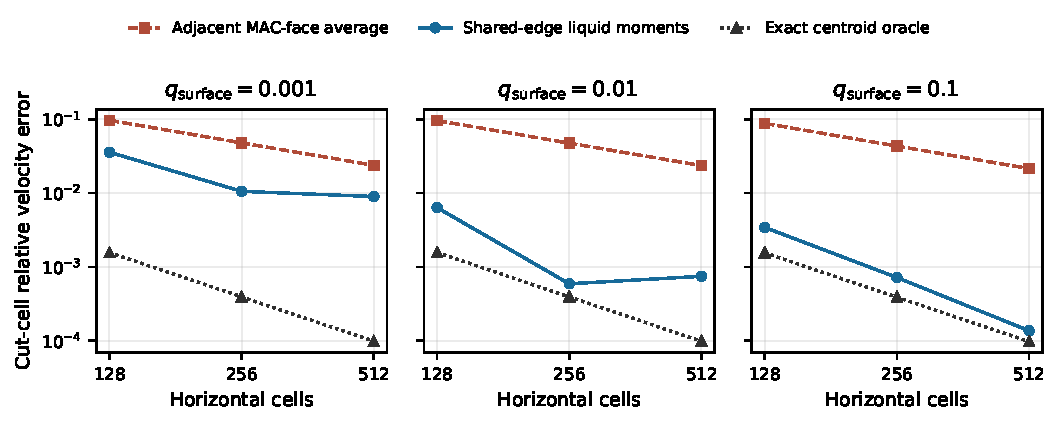
\includegraphics[width=\linewidth]{figures/flat_sliver_comparison.pdf}
\caption{Flat-boundary stress tests before native projection. The prescribed
surface fraction is shown above each panel; the error norm includes both
cut rows. The L reconstruction improves on adjacent-face averaging,
but the exact-field centroid control is more accurate in all nine cases.}\label{fig:slivers}
\end{figure}

Figure~\ref{fig:slivers} shows how cut-cell accuracy depends on liquid
fraction. For $q_s=0.001$, the L cut-cell errors are
0.03585, 0.01057, and 0.008982. For $q_s=0.01$, they are 0.006350,
0.0005889, and 0.0007439, including a nonmonotone final step. At $q_s=0.1$,
the errors decrease from 0.003427 to 0.0007165 to 0.0001358. The analytic
centroid control is more accurate throughout, while simple MAC-face
averaging is less accurate. Liquid volume remains conserved to roundoff
in all cases. Thus conservation and improvement over arithmetic averaging
do not imply lower error than sampling the exact liquid-domain field, or
uniform second-order behaviour in thin liquid regions.

To isolate trace-sampling sensitivity, two additional runs increase the
number of boundary trace samples fourfold while holding the Cartesian grid
and the analytic domain fixed, with $q_s=0.001$. At 256 horizontal cells,
the cut-cell error decreases from 0.0105686 to 0.0087533; at 512 cells,
it decreases from 0.0089818 to 0.0007110. These are reductions by factors
1.21 and 12.63, respectively. The geometry remains exactly flat, and the
exact-field centroid control is unchanged. Thus trace resolution is a material source
of error, but this control does not establish that it is the only source
or that additional sampling yields uniform convergence as $q_s\to0$.

A comparison over all liquid cells uses the liquid-volume-weighted
norm in equation~\eqref{eq:l2}, rather than the unweighted cut-cell
norm in Figure~\ref{fig:slivers}. Across the same nine cases, the L
reconstruction reduces this global error by factors 4.30--27.05 relative
to arithmetic MAC averaging. However, its global errors are 4.61--27.39
times larger than those of the exact-field centroid control. Thus a global
accuracy advantage also depends on the comparator; conservation of an
integral does not establish superiority in a global velocity norm.

A surface-row-only norm confirms that the poor thin-cell result is not
caused by pooling the bed row. At 512 cells and
$q_s=0.001$, its L error decreases from 0.0093744 to 0.00073369
under fourfold trace refinement, compared with an unchanged exact-field centroid
error of 0.0001004. Conversely, for $q_s=0.1$ on the finest original grid,
the L surface-row error is $8.7735\times10^{-5}$, slightly below the
control error. This local exception does not change the ranking of the
pooled cut-cell norm in Figure~\ref{fig:slivers}.

\subsection{Fixed overturning-wave state}
Before the native-bed adjustment, the fixed wave state satisfies the
offline volume and momentum checks on all three receiver grids
(Table~\ref{tab:transfer}). Native loading on the matched geometry is
reported separately below. The repeated momentum error reflects shared
boundary data and does not establish convergence with receiver spacing.
Near-boundary point probes and liquid-volume means measure different quantities.

\begin{table}[htbp]\centering\small
\caption{Offline transfer measurements on the pre-adjustment polygon
geometry, before loading into the receiver.
MAC divergence is the full Cartesian
identity before native receiver loading. Probe errors are pointwise-reference
relative $L^2$ measurements.}\label{tab:transfer}
\begin{tabular}{lrrrr}\toprule
Grid & $e_V$ & $e_M$ & MAC divergence $L^\infty$ & Probe error\\\midrule
L10 & $1.75\,10^{-16}$ & $6.96\,10^{-8}$ & $1.78\,10^{-15}$ & $7.67\,10^{-3}$\\
L11 & $1.75\,10^{-16}$ & $6.96\,10^{-8}$ & $3.55\,10^{-15}$ & $1.29\,10^{-3}$\\
L12 & $1.75\,10^{-16}$ & $6.96\,10^{-8}$ & $7.11\,10^{-15}$ & $1.07\,10^{-3}$\\
\bottomrule\end{tabular}
\end{table}

Independent BIE volume integration was performed for 12 cells selected by
geometry alone with $0.05<q_K<0.95$. The sampled relative velocity
error is $7.2115\times10^{-4}$, while the reported quadrature disagreement is
$1.5248\times10^{-8}$. Close evaluation uses source refinement and a common
potential-gauge subtraction on both boundaries. This test excludes sliver
cells and uses the geometry preceding the native-bed adjustment. We next
assess the reconstructed native geometry.

\subsection{Independent reference on native bed-cut cells}
Changing the represented bed and applying the volume-matching surface shift
also changes the reference-integration domain. It is invalid to use an
interior BIE formula indiscriminately outside its source domain. We therefore
check whether each native liquid polygon lies inside the declared source
polygon, allowing an area discrepancy no greater than $10^{-12}h^2$.
Of 8,495 native mixed cells, 3,479 satisfy this check and 5,016 do not;
the largest excluded area is $1.74993\times10^{-7}$ in one cell.
Containment in the source polygon is a numerical screening condition, not
a proof of containment in the continuously Fourier-refined BIE contour.

After checking that a centroid fan triangulates each simple polygon without
leaving it, six cells are selected deterministically
from each of the intervals $0.05<q<0.95$ and $0.95<q<1$.
The eligible populations are 3,150 and 134 cells. All 12 selected cells
intersect the bed, not the free surface; the source-domain screen excludes
many displaced free-surface polygons. The sample therefore tests native
bed-cut means and cannot establish accuracy over the whole free surface.
The reference is the fixed source BIE field integrated over these native
polygons; it is not a re-solved potential-flow problem on the receiver's
modified bed.

Independent BIE velocity evaluation is integrated with a radial Duffy map
on the centroid-fan triangles. The relative difference between three- and
five-point Gaussian rules is $2.26482\times10^{-10}$ at the original
source-evaluation tolerance. Because agreement between volume-quadrature
rules alone does not bound their common source-evaluation error, the
five-point reference is recomputed on the same cells with 100-fold
tighter source tolerances. This requires two successive source-refinement
agreements within $10^{-9}+10^{-7}\|\boldsymbol u\|_\infty$ per point.
All 1,225 quadrature points satisfy this criterion by a maximum source
resampling factor of 8,192. The relative change of the integrated reference
means is $6.81445\times10^{-11}$, well below the reconstruction errors.
Both reconstructions are compared with this stricter five-point reference
using the unweighted norm over the sampled cell means
(Table~\ref{tab:native-reference}).

\begin{table}[htbp]\centering\small
\caption{Independent reference for 12 selected native bed-cut cells.
Errors are unweighted relative Euclidean norms of phase-mean velocities.}
\label{tab:native-reference}
\begin{tabular}{lrrr}\toprule
Liquid-fraction interval & Cells & L moments & Bilinear-centroid control\\\midrule
$(0.05,0.95)$ & 6 & $4.82343\,10^{-6}$ & $1.77693\,10^{-4}$\\
$(0.95,1)$ & 6 & $2.07174\,10^{-5}$ & $2.88663\,10^{-5}$\\
Pooled sample & 12 & $1.61051\,10^{-5}$ & $1.17025\,10^{-4}$\\
\bottomrule\end{tabular}
\end{table}

The pooled L error is smaller by a factor of 7.27. It is smaller in
nine individual cells, whereas the control is more accurate in three.
This sampled comparison does not cover the thinnest liquid cells. An
attempted four-cell BIE reference for thinner cells failed the close-evaluation
criterion at 11 of 144 quadrature points, all in two cells with
$q=0.0003553$ and $q=0.03266$; those points are excluded from the accuracy
comparison. Thin cells are assessed with the analytic flat-boundary test.

\subsection{Receiver geometry and startup}
Table~\ref{tab:geometry} isolates the effect of receiver-matched geometry.
The original preparation had the prescribed offline liquid volume but lost
liquid when loaded. The measured loss is explained by clipping against the
different native solid geometry. Matching the receiver convention removes
that discrepancy to roundoff for the tested state.

\begin{table}[htbp]\centering\small
\caption{Geometry consistency and liquid-volume loss at loading.}
\label{tab:geometry}
\begin{tabular}{lrr}\toprule
Measurement & Polygon-only & Receiver-matched\\\midrule
Maximum offline/native $c_s$ difference & $7.17409\,10^{-4}$ & $9.37028\,10^{-14}$\\
Relative initial mass error & $1.19487\,10^{-7}$ & $1.75329\,10^{-16}$\\
Relative initial momentum error & $8.89928\,10^{-8}$ & $6.96337\,10^{-8}$\\
\bottomrule\end{tabular}
\end{table}

The matched L12 input reaches $t=0.01$ in 33 steps. At the final state the
relative physical liquid-volume change
is $8.76644\times10^{-16}$ and the embedded volume-flux divergence
$L^\infty$ is $3.16902\times10^{-12}$. The reported liquid-regular and
all-cell maximum speeds are 1.83611 and 2.52053. The former uses the
mask $c_s\ge0.5$, $f>0.01$ and does not bound every small embedded cell.
The measured wall time, 225.505 seconds, includes 21 checkpoint commits;
it is not a transfer-only cost or a speedup comparison.

\subsection{Paired native initialisations}
Both L12 branches complete the exact common interval $0\le t\le0.01$.
Their input phase moments differ:
the L relative momentum error is $6.96337\times10^{-8}$, about
15.8 times smaller than the uncorrected bilinear-centroid control's error.
This improves the initial integral constraint; subsequent accuracy requires
an independent evolved reference.
Table~\ref{tab:native-pair} reports the branch differences at the initial
and final common times.

\begin{table}[htbp]\centering
\caption{Difference between the two native branches at identical times.
These are sensitivity measurements, not errors against an exact flow.}
\label{tab:native-pair}
\begin{tabular}{lrr}\toprule
Measurement & $t=0$ & $t=0.01$\\\midrule
Liquid velocity difference $D_u$ & $9.37400\,10^{-4}$ & $9.48721\,10^{-4}$\\
VOF fraction difference $D_f$ & 0 & $4.37319\,10^{-5}$\\
Column liquid-depth difference $D_H$ & 0 & $5.80190\,10^{-6}$\\
Relative liquid-volume difference & 0 & $5.25987\,10^{-16}$\\
\bottomrule\end{tabular}
\end{table}

At $t=0.01$, the density-normalised liquid kinetic energies
$\tfrac12h^2\sum_Kq_K\|\boldsymbol u_K\|_2^2$ are 0.43967054
and 0.43969504 for the L and control branches. The maximum column-depth
difference is $1.16104\times10^{-4}$. The receiver thus retains some
sensitivity to the input moment operator, while liquid volume agrees to
roundoff. An independent evolved reference is needed to rank their accuracy.

\subsection{Time-step sensitivity}\label{app:time-step}
A second paired experiment halves the initial step limit from 0.00125 to
0.000625, the maximum step from 0.000625 to 0.0003125, and both CFL controls
from 0.05 to 0.025. Each full-step branch takes 32 steps and each
half-step branch takes 64 steps to reach $t=0.01$. These runs use a different
step schedule from the 33-step startup above. Table~\ref{tab:timestep} uses the same relative norms,
with the first-listed state supplying the denominator and liquid weights.

\begin{table}[htbp]\centering\small
\caption{Endpoint sensitivity to one time-step halving.}
\label{tab:timestep}
\begin{tabular}{lrr}\toprule
Comparison at $t=0.01$ & $D_u$ & $D_f$\\\midrule
Full-step L versus control & $9.48721\,10^{-4}$ & $4.37319\,10^{-5}$\\
Half-step L versus control & $9.58218\,10^{-4}$ & $4.28176\,10^{-5}$\\
L full versus half step & $5.13667\,10^{-3}$ & $1.21956\,10^{-4}$\\
Control full versus half step & $5.15092\,10^{-3}$ & $1.22843\,10^{-4}$\\
\bottomrule\end{tabular}
\end{table}

The branch differences change little under this halving, but the
full-versus-half-step differences are larger than the differences between
initialisations. Thus the experiment detects a persistent short-time
influence of the transfer operator without establishing temporally resolved
dynamic superiority. Two time settings do not establish a convergence
order or an error against the physical trajectory.

\subsection{Propagation and boundary-trace resolution}
This separate smooth-wave test increases the boundary-trace factor from 8
to 32 for both L and B, keeping the 512 source nodes and physical geometry
fixed. The exact-input reference, liquid fractions, embedded geometry and
gas velocities remain fixed. Recomputed preprocessing face velocities change
only at numerical-noise scale; the serialized common face arrays are copied
unchanged from the original reference. Native face fluxes are reconstructed
separately from each branch's cell velocities. For this flat surface, the
streamfunction trace is $-A\tanh(kD)\sin(kx)$, with maximum second
derivative 0.04487475. Its original and refined spacings are $1/64$ and
$1/256$. For upper liquid-strip height $q_Kh=6.25\times10^{-5}$,
Eq.~\eqref{eq:trace-bound} bounds the isolated physical-trace contribution
by 0.02191 and 0.001369, respectively; these are bounds on one error
component, not estimates of the total transfer or evolved error.

A further $2048\times128$ joint-refinement check uses trace factor 64,
preserving $\delta\sigma/h=1/16$ from the denser-trace $1024\times64$
case. The 512 source nodes, geometry, potential amplitude, wave mode and
endpoint remain fixed; the upper-row liquid fraction becomes 0.002. This
case uses only the full time-step limit. Time-step halving covers both
original-trace grids and the denser-trace $1024\times64$ case; no half-step
trajectory is inferred for untested cases.

The smooth native benchmark separates a global initial norm from the later
influence of that error. With the original trace factor, L transfer
has a smaller initial global error on the $512\times32$ grid, but its error
at $0.1T$ is 2.88 times the bilinear control's error. On $1024\times64$, the
initial L error is already 4.31 times larger and the endpoint error is
10.19 times larger. Thus a small initial global norm, like a closed global
moment balance, does not ensure a better subsequent state.
Figure~\ref{fig:dynamics} compares the corresponding error histories and
the effect of increasing the trace density. Its vertical axes are logarithmic.

\begin{figure}[tbp]\centering
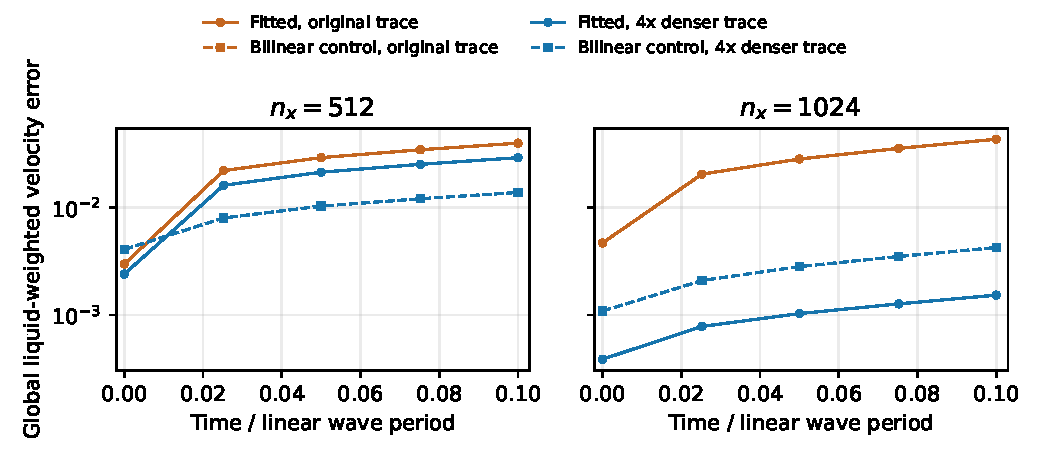
\includegraphics[width=\linewidth]{figures/native_transfer_dynamics.pdf}
\caption{Native propagation of initial transfer error for the smooth-wave
benchmark, using the full time-step limit. Each curve is measured against
the same-grid native branch initialised with exact liquid-cell means.
The two trace densities give practically coincident bilinear-control
curves. The refined L transfer improves the finer-grid result but
still loses to the control on the coarse grid. This is not an error plot
against an exact two-phase trajectory.}\label{fig:dynamics}
\end{figure}

The trace-density intervention keeps source values, geometry, gas fields
and reference inputs fixed. The computed streamfunction changes by only
$4.65\times10^{-13}$ and $1.39\times10^{-12}$ in relative norm at the two
grids, while a L wet-cell velocity component changes by as much as
0.0136; recomputed preprocessing MAC face velocities change by at most
$2.15\times10^{-12}$.
Together with the unchanged liquid fractions, this localises the main
change to boundary-trace and edge-moment reconstruction, including trace
values at boundary intersections, rather than geometry or the bulk harmonic
solve. The data do not isolate physical-edge integrals from all other
boundary-dependent edge terms. In the original $1024\times64$ input, 99.43\% of the L
squared liquid-weighted velocity error is in the upper thin liquid row.

On $1024\times64$, fourfold trace refinement lowers the L initial
error from $4.69958\times10^{-3}$ to $3.8820\times10^{-4}$.
At $0.1T$, its global velocity error is $1.53448\times10^{-3}$, compared
with $4.25970\times10^{-3}$ for the same-streamfunction bilinear control:
a 2.78-fold reduction. The relative VOF errors are $5.31475\times10^{-6}$
and $2.14689\times10^{-5}$. Normalising the column-depth error by the
reference wave component $\|H^R-\langle H^R\rangle\|_2$, rather than the
background depth, gives $1.34113\times10^{-4}$ and $5.41771\times10^{-4}$,
a 4.04-fold reduction. The maximum absolute column-depth differences are
$2.518\times10^{-6}$ and $9.111\times10^{-6}$. The reference wave's mode-16
amplitude is 0.01396. These measurements demonstrate a reduced propagated
transfer error in this finer-grid case.

The coarse-grid result remains unfavourable: refined L and control
velocity errors are $2.92106\times10^{-2}$ and $1.38609\times10^{-2}$.
The density intervention therefore does not establish a grid-independent
advantage or a uniform small-cell accuracy guarantee.

The favourable $1024\times64$ comparison survives one time-step halving:
the L and control velocity errors become $1.59996\times10^{-3}$ and
$4.46877\times10^{-3}$, giving a 2.79-fold reduction. Their wave-normalised
column-depth errors are $1.48757\times10^{-4}$ and $6.34783\times10^{-4}$,
a 4.27-fold reduction. The logs record final zero-based step indices
210 and 420: 211 and 421 time advances, respectively. Each run takes
210 or 420 full steps of 0.0025 or 0.00125, followed by a shortened
final step of approximately $7.18\times10^{-5}$. The corresponding unrefined-trace
comparison remains unfavourable by a factor of 10.18.

The transfer ranking persists under this step halving, but temporal
convergence of the exact-input reference is not established. Its full-versus-half-step velocity
difference is $2.04241\times10^{-2}$, larger than the L-versus-reference
differences at either time setting. The primary ratios therefore quantify
the propagation of initialisation error under a common numerical evolution,
not the total error against a physical wave solution.

A further comparison uses the half-step exact-input branch as the common
reference for both full-step candidates. Their velocity discrepancies are
0.0209794 (L) and 0.0193803 (control): the L result is 8.3\% worse.
Thus the favourable matched-step ratios cannot be promoted to an assertion
of improved total trajectory accuracy. Common temporal error and its
interaction with initialisation dominate this cross-step comparison.
On $512\times32$ with the refined trace, the cross-step velocity ranking
also changes: discrepancies are 0.0204883 (L) and 0.0223687 (control),
whereas wave-normalised column-depth discrepancies are 0.00362516 and
0.00354270. The matched-step transfer ranking therefore does not extend
to this cross-step comparison.

The ranking reversal can be resolved algebraically without treating the
half-step trajectory as an exact physical reference. Let $u_m^{\Delta t}$
denote a transferred branch, $u_*^{\Delta t}$ the exact-input branch, and
$u_*^{\Delta t/2}$ the latter branch at the smaller step. With a single
liquid-volume inner product weighted by the half-step reference, define
$e_m=u_m^{\Delta t}-u_*^{\Delta t}$ and
$b=u_*^{\Delta t}-u_*^{\Delta t/2}$. Then
\begin{equation}
 \|u_m^{\Delta t}-u_*^{\Delta t/2}\|^2
 =\|e_m\|^2+\|b\|^2+2\langle e_m,b\rangle.
 \label{eq:temporal-error-decomposition}
\end{equation}
At the common endpoint of the refined $1024\times64$ case, the normalised
transfer norms are 0.00153846 and 0.00427009 for L and control inputs,
while $\|b\|/\|u_*^{\Delta t/2}\|=0.02042411$. The corresponding error-vector
cosines are $+0.3282$ and $-0.3427$. Thus the smaller control discrepancy
against the half-step reference includes cancellation of temporal error;
it does not by itself demonstrate a more accurate physical trajectory.
The squared-norm identity holds for the endpoint fields
to an absolute normalised residual below $4.4\times10^{-19}$.
These norms differ slightly from the matched-step values because their
weights and normalising reference are held fixed to the half-step branch.

The $2048\times128$ joint-refinement check gives the same matched-step
ranking. Initial L and control errors are
$1.03094\times10^{-4}$ and $3.34981\times10^{-4}$. At $0.1T$, their global
velocity errors are $5.08178\times10^{-4}$ and $1.74890\times10^{-3}$,
a 3.44-fold reduction. Wave-normalised column-depth errors are
$4.7457\times10^{-5}$ and $1.66515\times10^{-4}$, a 3.51-fold reduction.
All three branches complete 211 time advances (final step index 210); maximum recorded post-start
embedded-volume flux divergence is $8.10\times10^{-14}$ and recorded mass
drift is zero at output precision. This supports the matched-setting
transfer benefit at a second spatial resolution, but supplies no additional
time-step convergence evidence. Table~\ref{tab:dynamic-errors} retains the
complete tested matrix.

\begin{table}[tbp]\centering\small
\caption{Global propagated transfer errors at $t=0.1T$. The trace factor
is the number of trace samples per original source segment. Ratios
$R_u=E_u^{\rm control}/E_u^{\rm fitted}$ and $R_H$ for wave-normalised
column depth exceed one when the fitted transfer is better. Every
comparison uses a reference with the same grid and time-step limit.}
\label{tab:dynamic-errors}
\begin{tabular}{rrrrrrr}\toprule
$n_x$ & Trace & $10^3\Delta t_{\max}$ & $E_u^{\rm fitted}$ & $E_u^{\rm control}$ & $R_u$ & $R_H$ \\
\midrule
512 & 8 & 2.5 & 0.03988 & 0.01386 & 0.35 & 0.64 \\
512 & 8 & 1.25 & 0.04084 & 0.01419 & 0.35 & 0.60 \\
1024 & 8 & 2.5 & 0.04340 & 0.00426 & 0.10 & 0.13 \\
1024 & 8 & 1.25 & 0.04549 & 0.00447 & 0.10 & 0.14 \\
512 & 32 & 2.5 & 0.02921 & 0.01386 & 0.47 & 0.84 \\
1024 & 32 & 2.5 & 0.00153 & 0.00426 & 2.78 & 4.04 \\
1024 & 32 & 1.25 & 0.00160 & 0.00447 & 2.79 & 4.27 \\
2048 & 64 & 2.5 & 0.00051 & 0.00175 & 3.44 & 3.51 \\
\bottomrule\end{tabular}
\end{table}



\subsection{Earlier Matched continuations and time-step control}\label{app:old-matched}
These earlier M, B and exact-input continuations use the original receiver
build and trace factor~8. Within each $512\times32$ or $1024\times64$
comparison, geometry, volume fractions, supplied face data, gas velocities,
physical coefficients and full-step settings are common. All branches reach
$t=0.1T$ after 211 time advances (final step index 210). The receiver reconstructs runtime face fluxes from
each branch's cell velocities. These tests precede the corrected-build
three-grid series in Sections~\ref{sec:native-protocol} and~\ref{sec:dynamic-results}; their main value here
is the historical time-step control below.
Figure~\ref{fig:matched-dynamics} shows these earlier trajectories.

For completeness, the earlier endpoint M/B velocity errors are
0.00175849/0.01386093 on $512\times32$ and 0.000434603/0.004259703 on
$1024\times64$, reductions of 7.88 and 9.80. Their wave-normalised
surface-profile errors are $3.92627\times10^{-5}$/$2.55281\times10^{-3}$
and $7.33856\times10^{-6}$/$5.41771\times10^{-4}$, reductions of 65.0 and
73.8. The favourable ranking holds at every recorded nonzero time.
The M grid-refinement ratios are 4.015 initially and 4.046 at the endpoint
(observed two-grid orders 2.005 and 2.017); they do not establish
asymptotic convergence of the receiver.

Halving the time step on $1024\times64$ preserves the improvement.
The matched run completes 421 time advances (final step index 420)
and gives velocity error
0.0004361803 against the half-step exact-input branch, versus 0.0044687721
for the half-step B control (10.25-fold reduction). The respective
surface-profile errors are $7.65566\times10^{-6}$ and
$6.34783\times10^{-4}$ (82.9-fold reduction). The common receiver settings
are held fixed within each comparison; these ratios measure propagated
transfer error rather than the receiver's temporal truncation error.

The norms use $q_{\rm ref}=f_{\rm ref}c_{s,\rm ref}$ and
Eq.~\eqref{eq:dynamic-depth-error} on the output fields. Equal endpoint
times and common inputs isolate the transfer operator within each receiver
discretisation.

\begin{figure}[htbp]
\centering
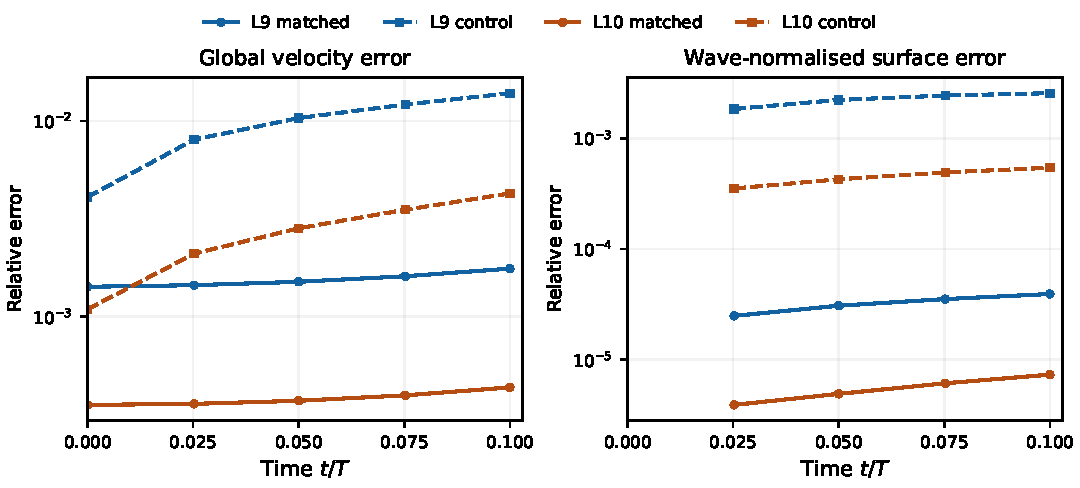
\includegraphics[width=\linewidth]{figures/matched_native_dynamics.pdf}
\caption{Propagation of transfer error on the original receiver build
with Matched (M) and Bilinear (B) initialisations. L9 and L10 denote $512\times32$ and
$1024\times64$ grids, both with $\Delta t_{\max}=0.0025$.
Each curve uses the exact-input numerical trajectory
at its own grid and identical time-step settings as the reference. The
surface error is undefined at the initially flat state and is shown only
at nonzero times.}\label{fig:matched-dynamics}
\end{figure}


\begin{thebibliography}{99}
\bibitem[Lachaume et al.(2003)]{lachaume}
C. Lachaume, B. Biausser, S. T. Grilli, P. Frauni\'e, and S. Guignard,
``Modeling of breaking and post-breaking waves on slopes by coupling of BEM
and VOF methods,'' in \emph{Proceedings of the 13th International Offshore
and Polar Engineering Conference}, 353--359 (2003).
\url{https://digitalcommons.uri.edu/oce_facpubs/177/}.
\bibitem[Colicchio et al.(2006)]{colicchio}
G. Colicchio, M. Greco, and O. M. Faltinsen,
``A BEM--level set domain-decomposition strategy for non-linear and fragmented
interfacial flows,'' \emph{International Journal for Numerical Methods in
Engineering} \textbf{67}, 1385--1419 (2006).
\url{https://doi.org/10.1002/nme.1680}.
\bibitem[Zhang and Buldakov(2025)]{zhang}
C. Zhang and E. Buldakov,
``Evaluating RANS and LES turbulence models in hybrid wave modelling of
breaking waves,'' \emph{Frontiers in Marine Science} \textbf{12}, 1484783 (2025).
\url{https://doi.org/10.3389/fmars.2025.1484783}.
\bibitem[Sun and Wheeler(2006)]{sun}
S. Sun and M. F. Wheeler, ``Projections of velocity data for the compatibility
with transport,'' \emph{Computer Methods in Applied Mechanics and Engineering}
\textbf{195}, 653--673 (2006).
\url{https://doi.org/10.1016/j.cma.2005.02.011}.
\bibitem[Ullrich and Taylor(2015)]{ullrich}
P. A. Ullrich and M. A. Taylor,
``Arbitrary-order conservative and consistent remapping and a theory of linear
maps: Part I,'' \emph{Monthly Weather Review} \textbf{143}, 2419--2440 (2015).
\url{https://doi.org/10.1175/MWR-D-14-00343.1}.
\bibitem[Chang et al.(2019)]{chang}
J. Chang, V. C. Azevedo, and C. Batty,
``Divergence-free and boundary-respecting velocity interpolation using stream
functions,'' in \emph{ACM SIGGRAPH/Eurographics Symposium on Computer Animation},
article 7, 1--2 (2019).
\url{https://doi.org/10.1145/3309486.3339890}.
\bibitem[Chang et al.(2022)]{curlflow}
J. Chang, R. Partono, V. C. Azevedo, and C. Batty,
``Curl-Flow: Boundary-respecting pointwise incompressible velocity
interpolation for grid-based fluids,'' \emph{ACM Transactions on Graphics}
\textbf{41}(6), 243:1--243:21 (2022).
\url{https://doi.org/10.1145/3550454.3555498}.
\bibitem[Overton-Katz et al.(2023)]{overton}
N. Overton-Katz, X. Gao, S. Guzik, O. Antepara, D. T. Graves, and
H. Johansen, ``A fourth-order embedded boundary finite volume method
for the unsteady Stokes equations with complex geometries,''
\emph{SIAM Journal on Scientific Computing} \textbf{45}, A2409--A2430 (2023).
\url{https://doi.org/10.1137/22M1532019}.
\bibitem[Rudman(1998)]{rudman}
M. Rudman, ``A volume-tracking method for incompressible multifluid flows
with large density variations,'' \emph{International Journal for Numerical
Methods in Fluids} \textbf{28}, 357--378 (1998).
\url{https://doi.org/10.1002/(SICI)1097-0363(19980815)28:2<357::AID-FLD750>3.0.CO;2-D}.
\bibitem[Arrufat et al.(2021)]{arrufat}
T. Arrufat, M. Crialesi-Esposito, D. Fuster, Y. Ling, L. Malan, S. Pal,
R. Scardovelli, G. Tryggvason, and S. Zaleski,
``A mass-momentum consistent, Volume-of-Fluid method for incompressible
flow on staggered grids,'' \emph{Computers \& Fluids} \textbf{215}, 104785 (2021).
\url{https://doi.org/10.1016/j.compfluid.2020.104785}.
\bibitem[Weymouth and Yue(2010)]{weymouth}
G. D. Weymouth and D. K.-P. Yue,
``Conservative Volume-of-Fluid method for free-surface simulations on
Cartesian-grids,'' \emph{Journal of Computational Physics}
\textbf{229}, 2853--2865 (2010).
\url{https://doi.org/10.1016/j.jcp.2009.12.018}.
\bibitem[Gibou et al.(2002)]{gibou}
F. Gibou, R. P. Fedkiw, L.-T. Cheng, and M. Kang,
``A second-order-accurate symmetric discretization of the Poisson equation
on irregular domains,'' \emph{Journal of Computational Physics}
\textbf{176}, 205--227 (2002).
\url{https://doi.org/10.1006/jcph.2001.6977}.
\bibitem[Karnakov et al.(2020)]{karnakov}
P. Karnakov, F. Wermelinger, S. Litvinov, and P. Koumoutsakos,
``Aphros: High performance software for multiphase flows with large scale
bubble and drop clusters,'' in \emph{Proceedings of the Platform for Advanced
Scientific Computing Conference (PASC '20)} (ACM, 2020), 1--10.
\url{https://doi.org/10.1145/3394277.3401856}.
\bibitem[Aphros developers(2026)]{aphros}
Aphros developers, \emph{Aphros documentation: embedded boundaries and
volume-of-fluid solvers}. Accessed 30 September 2026.
\url{https://cselab.github.io/aphros/doc/index.html}.
\bibitem[Fitzpatrick(2016)]{fitzpatrick}
R. Fitzpatrick, ``Surface tension,'' in \emph{Fluid Mechanics lecture notes}
(University of Texas at Austin, 2016). Accessed 1 October 2026.
\url{https://farside.ph.utexas.edu/teaching/336L/Fluidhtml/node156.html}.
\bibitem[Baturin(2026)]{baturin-transfer}
S. Baturin, \emph{Geometry-consistent conservative transfer of potential-flow
states to an embedded-boundary volume-of-fluid solver: code and numerical
experiments}, version v0.31.0 (Zenodo, 2026).
\url{https://doi.org/10.5281/zenodo.23104557}.
\bibitem[Baturin(2026b)]{baturin-followup}
S. Baturin, \emph{Geometry-consistent conservative transfer of potential-flow
states to an embedded-boundary volume-of-fluid solver: code and numerical
experiments}, version v0.32.0 (Zenodo, 2026).
\url{https://doi.org/10.5281/zenodo.23111007}.
\end{thebibliography}
\end{document}
